\PassOptionsToPackage{unicode}{hyperref}
\documentclass[aspectratio=1610, 9pt]{beamer}

% Load packages you need here
\usepackage{polyglossia}
\setmainlanguage{english}

\usepackage{csquotes}
    

\usepackage{amsmath}
\usepackage{amssymb}
\usepackage{mathtools}

\usepackage{hyperref}
\usepackage{bookmark}

% load the theme after all packages

\usetheme[
  showtotalframes, % show total number of frames in the footline
]{tudo}

% Put settings here, like
\unimathsetup{
  math-style=ISO,
  bold-style=ISO,
  nabla=upright,
  partial=upright,
  mathrm=sym,
}

\title{Generation and time-resolved detection of
terahertz radiation}
\author[M.~Koch]{Max Koch}
\institute[AG Wang]{Arbeitsgruppe Wang \\  Fakultät Physik}
\titlegraphic{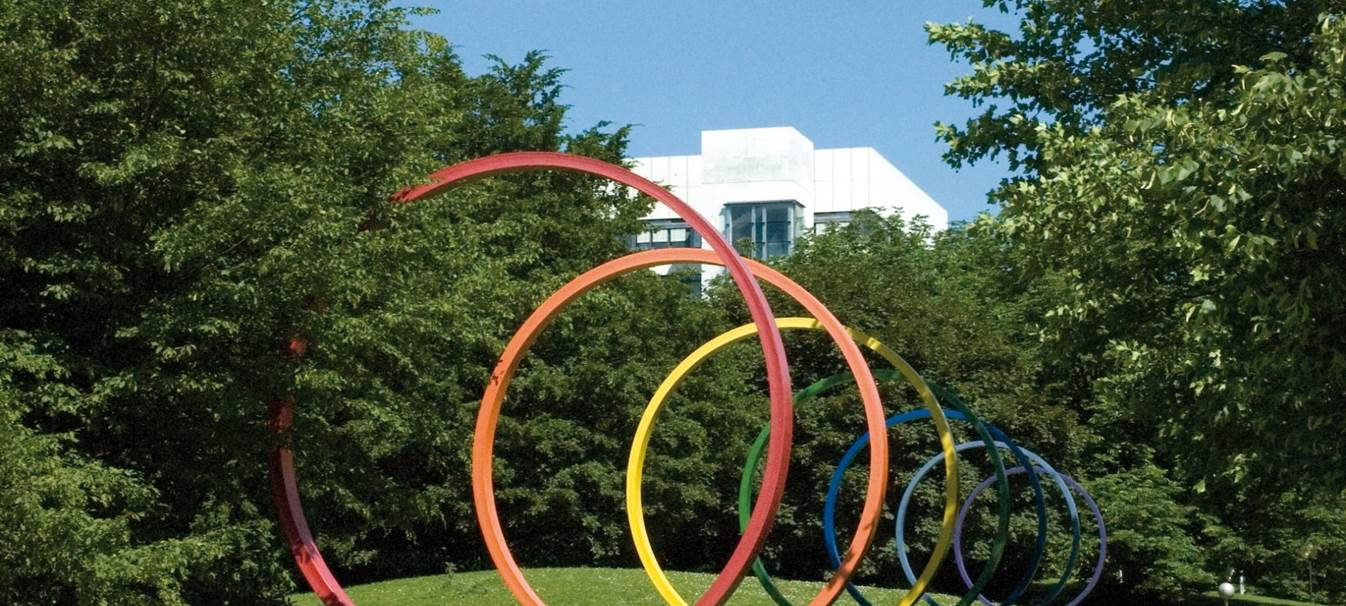
\includegraphics[width=0.7\textwidth]{images/tudo-title-2.jpg}}


\begin{document}

\maketitle

\chapter{Introduction}
For many applications the spectroscopy is an easy and efficient way to explore the properties of diffrent materials.
That is why the spectroscopy finds applications in many fields, from biology and medizin to physics and engeneering.
A big leap in the science of spectroscopy was made in 1895 when Wilhelm Conrad Röntgen first discovered the X-Ray radiation \cite{roentgen}.
With this new form of electromagnetic radiation many new applications in medizin and physics evolved and a new area of spectroscopy began.
Over the years more and more sources and detectors of various electromagnetic radiation were developed.
But for long there was still a gap in the spectrum.
It is known as the terahertz gap and describes the incapability of producing terahertz radiation form around $0.3-10\,\si{\tera\hertz}$ in an efficient and easy way \cite[157--159]{THzgap_applications}.
Since some years there have been efforts to close the terahertz gap and develope methodes of producing terahertz radiation.
The reason for this is that terahertz radiation has some interesting properties that would be of interest for diffrent fields.
Its non ionizing properties make it of particular interest in diffrent areas of medizin, because it does not have an harming effect on tissue\cite[161--162]{THzgap_applications}.
For instence in dermatology, where terahertz imaging processes can be used to determine the moisture content of the skin or might even give diagnostic methodes to detect skin cancer\cite{terahertz_dermatology}. 
Because of the same reason, and a specific spectroscopic fingerprint for most metals, the terahertz radiation is also of interest in the security sector.
Weapons like guns, knifes and even most soft explosives can be detected using terahertz spectroscopy \cite[162]{THzgap_applications}\cite{thz_explosive_detec}.
In 1995-1996 an advance in the production of wide bandwidth terahertz radiation was made by using electro-optic sampling in non linear crystals such as zinc telluride \cite{first_eos_wu_zhang}\cite{ZnTe_Nahata_Weling_1996}.


This thesis concentrates on the production of terahertz radiation through electro-optic sampling with a zinc telluride crystal.
% Three times the,      I should try to get a better formulation here.
The produced radiation is then refelected and focused into another zinc telluride crystal, in which the terahertz electric field induces a birefringence.
The birefringence then effects the polarization of the probe beam which hits the detector zinc telluride crystal roughly at the same time as the terahertz beam.
The timing of the terahertz beam can be changed by manipulating the beam path length with a delay stage.
This way the whole time domain of the tera hertz beam can be probed.
% For terahertz spectroscopy of probes two additional mirrors are added to focus the radiation onto a probe, before it is then focused into the detection crystal.
After the probe beam passed through the detection crystal, its split into its two polarizations components which are observered by a photodiode.
The signal of both photodiodes then show how much the terahertz beam affected the polarization of the probe beam which shows how strong the electric field of the terahertz beam was.
This setup was first demonstrated by Nahata A., Weling A. S., and Heinz T. F. in 1996 \cite{ZnTe_Nahata_Weling_1996}.





% %%%%%%%%%%%%%%%%%%%%%%%%%%%%%%%%%%%%%%%%%%%%%%%%%%%%%%%%
% Für viele Anwendungen ist die Spektroskopie eine der effizientesten Möglichkeiten um gewisse Materialeigenschaften einer Probe zu bestimmen.
% So haben die Wissenschaftler in vielen Bereichen auf die Methode zurück gergriffen und von ihrer relativen einfachen Umsetzung profitiert.
% Ein großer Durchbruch in dem Bereich der Spektroskopie ist der Physik gelangt als Wilhelm Conrad Röntgen 1895 %(Entdeckung Röntgen Strahlung)
% die Röntgenstrahlen entdeckt hat.
% Durch diese neue Form der Strahlung konnte die Wissenschaft in neue Bereiche eintreten.
% Über die Jahre wurden dem Spektrum mit dem Spektroskopie möglich ist immer neue Strahlungsarten hinzugefügt.
% Doch eine Lücke im Spektrum besteht bis heute.
% Sie ist als THz-Lücke bekannt und bezeichnet die bis heute noch ineffieziente und relativ komplizierte Produktion von THz-Strahlung und Detektion.
% Seit einigen Jahren werden nun immer mehr Bestrebungen daran gesetzt diese Lücke zu schließen.
% Denn THz Strahlung ist für verschiedene wissenschaftliche Bereiche von großem Interesse.
% So könnten in der Medizin neue Methoden zur Dutchleuchtung organischer Materie entwickelt werden ohne das die Materie dabei durch Ionisierung zerstört wird.
% Des weiteren ist sie auch für die Physik vom großem Interesse da durch elektromagnetische Wellen im THz-Frequenz bereich bestimme Gitterschwingungen angeregt werden.
% Ein großer Durchbruch gelang als 1996 das erste mal THz durch optical rectification in anorganischen Kristallen erzeugt wurde. %\cite{ZnTe_Nahata_Weling_1996}
% Dieser Durchbruch gelang durch das bestrahlen eines Zinc Telluride Kristalls mit einem Laser in 800 nm Bereich.
%%%%%%%%%%%%%%%%%%%%%%%%%%%%%%%%%%%%%%%%%%%%%%%%%%%%%%%%%%
% Motivation
% Hier folgt eine kurze Einleitung in die Thematik der Bachelorarbeit.
% Die Einleitung muss kurz sein, damit die vorgegebene Gesamtlänge der 
% Arbeit von 25 Seiten nicht überschritten wird. 
% Die Beschränkung der Seitenzahl sollte man ernst nehmen,
% da Überschreitung zu Abzügen in der Note führen kann. 
% Um der Längenbeschränkung zu genügen, darf auch nicht an der Schriftgröße,
% dem Zeilenabstand oder dem Satzspiegel (bedruckte Fläche der Seite) manipuliert werden.


\input{content/02_theorie.tex}
\chapter{Setup}\label{make}

\chapter{Results}
This section will present the results of the measurements with ZnTe and GaP as emitter crystals.
Calculations will be made to determine the electric field strength of the generated $\si{\tera\hertz}$ radiation as well as the power of said radiation.
Further, a comparison between the different spectrums of ZnTe and GaP will be shown.
The efficiency of producing radiation will be discussed.

\section{Zinc telluride}
For these measurements, a $\SI{1}{\milli\meter}$ thick ZnTe crystal is used as the emitter.
Another $\SI{1}{\milli\meter}$ thick ZnTe crystal is used as the detector.
The measurements are taken as described in section \ref{sec:execution}.
At this point, it should be mentioned, that the ZnTe crystal that is used as the emitter has two burn marks on it.
\\
The burned crystal can be seen in figure \ref{fig:ZnTe_burned}.
The burned part of the crystal harms the efficiency of $\si{\tera\hertz}$ generation.
This is why the part of the laser with the highest power is not focused on the burned part.
Still, some of the laser's power hits the burned part of the crystal.
\\\\
To understand the data, the first figure that is examined is the time-resolved EOS data.
For this, the lock-in amplifier output is plotted against the time delay between the pump and probe beam.
Figure \ref{ZnTe:2_11_30_20_signal} shows the resulting plot.
This measurement is taken with a pump power of $\SI{135.0}{\milli\W}$, which is the highest pump power that is used.
The typical trend of a $\si{\tera\hertz}$ pulse can be seen.
\begin{figure}
    \centering
    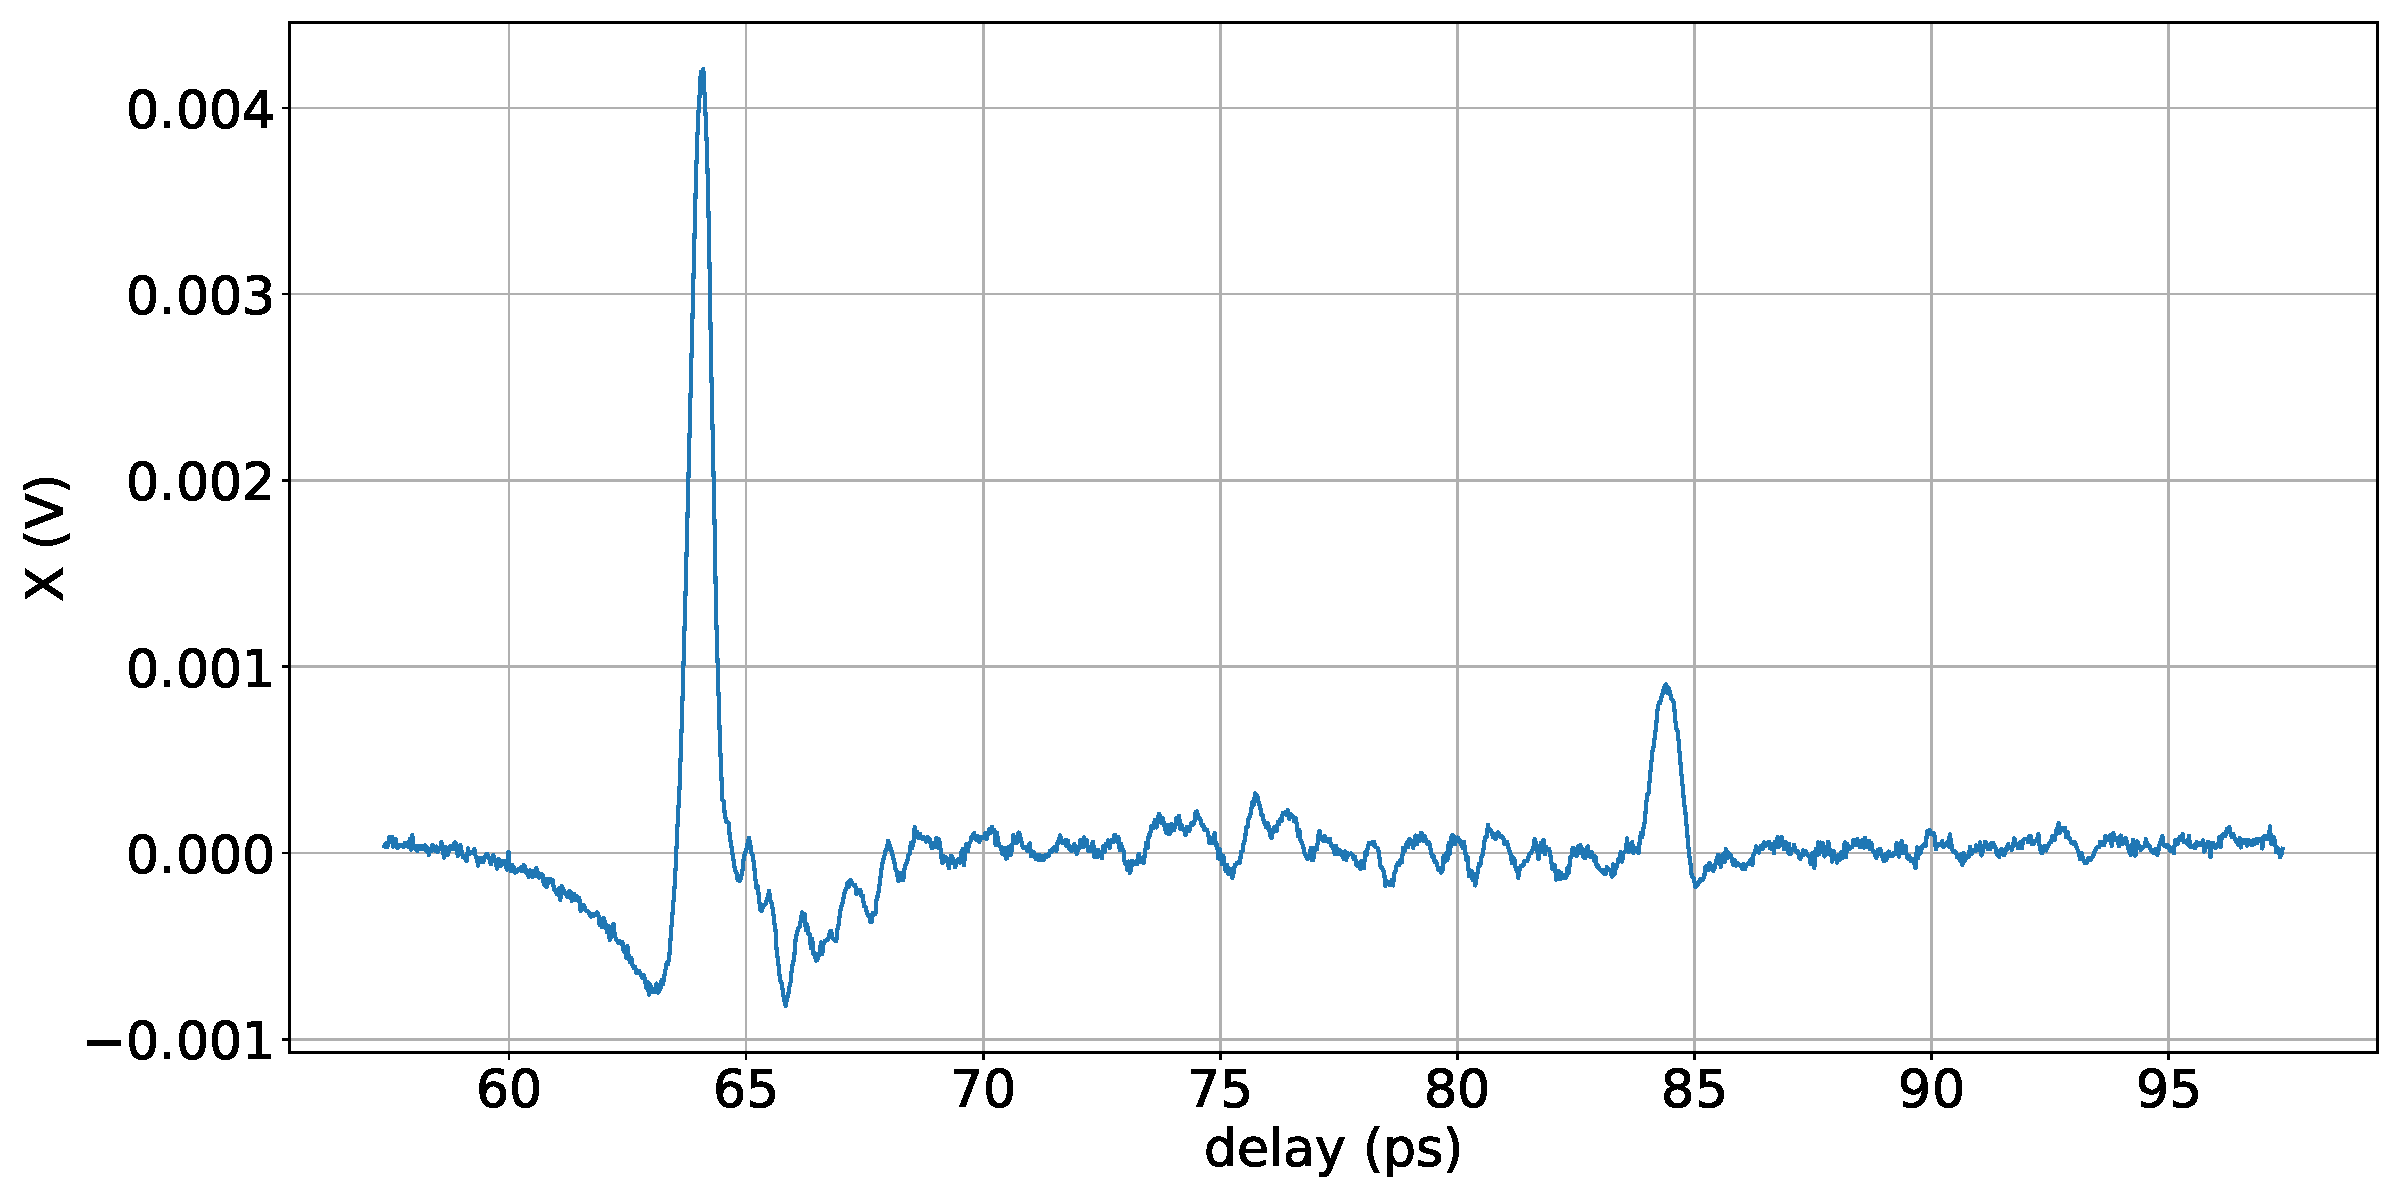
\includegraphics[width=0.8\textwidth]{Plots/2_11_30_20normalX.pdf}
    \caption{The $\si{\tera\hertz}$ pulse generated by ZnTe, which is measured by EOS, with a pump power of $\SI{135.0}{\milli\W}$.
    The EOS signal is plotted against the delay in $\si{\pico\second}$.
    A post pulse can be seen at a delay of $\SI{84}{\pico\second}$.}
    \label{ZnTe:2_11_30_20_signal}
\end{figure}
\FloatBarrier
Before the pulse starts the signal is balanced at $X(V)=0$.
At a delay of about $\SI{58}{\pico\second}$ the pulse starts, which manifests in an increasingly negative $X(V)$ value.
After about $\SI{5}{\pico\second}$ behind the start, the minimum is reached with an $X(V)$ value of $\SI{-0.746}{\milli\V}$ after which the lock-in amplifier output increases up to a value of $\SI{4.206}{\milli\V}$.
Here the maximum of the plot is reached, which corresponds to the maximum $\si{\tera\hertz}$ electric field strength inside the detector crystal.
After the maximum, the signal drops almost to zero.
\\
From this point on there are some oscillations, but no major features are visible. %are those oscillations acuatlly caused by water?
Up until a delay of $\SI{84}{\pico\second}$, where the post pulse starts.
The post pulse is caused by reflections of the $\si{\tera\hertz}$ pulse inside the crystal.
This is why the post pulse is just an echo of the initial pulse and thus alters the signal in a negative way.
For further calculations, the data that is taken up until the post pulse will be used.
\\\\
To confirm that the pulse that is shown in figure \ref{ZnTe:2_11_30_20_signal} corresponds to a $\si{\tera\hertz}$ pulse a Fourier-Transformation of the data is calculated. %Do I need to mention FFT in theory?
Because the Fourier-Transformation is done numerically the FFT function of the python package scipy \cite{scipy} is used.
The resulting Fourier spectrum is shown in figure \ref{fig:2_11_30_20_fft}.
\\
The spectrum is also plotted against a logarithmic y-axis, which results in the plot in figure \ref{fig:2_11_30_20_fft_log}.
\\\\
With this, it is easy to confirm that the generated radiation lies in the $\si{\tera\hertz}$ regime.
Furthermore, most of the radiation that is generated has a frequency between $0.3-1.1\,\si{\tera\hertz}$, but radiation with even higher $\si{\tera\hertz}$ frequencies is generated as well.
Especially in the spectrum which is plotted against the logarithmic y-axis the water absorption line of $\SI{1.226}{\tera\hertz}$ is visible \cite{water_absorption}.
This is due to the water vapor in the air between the emitter and detector crystal.
Some features at even higher frequencies are visible too, which might be additional absorption lines.
\begin{figure}%
    \centering
    \begin{subfigure}{.55\textwidth}%
        \centering
        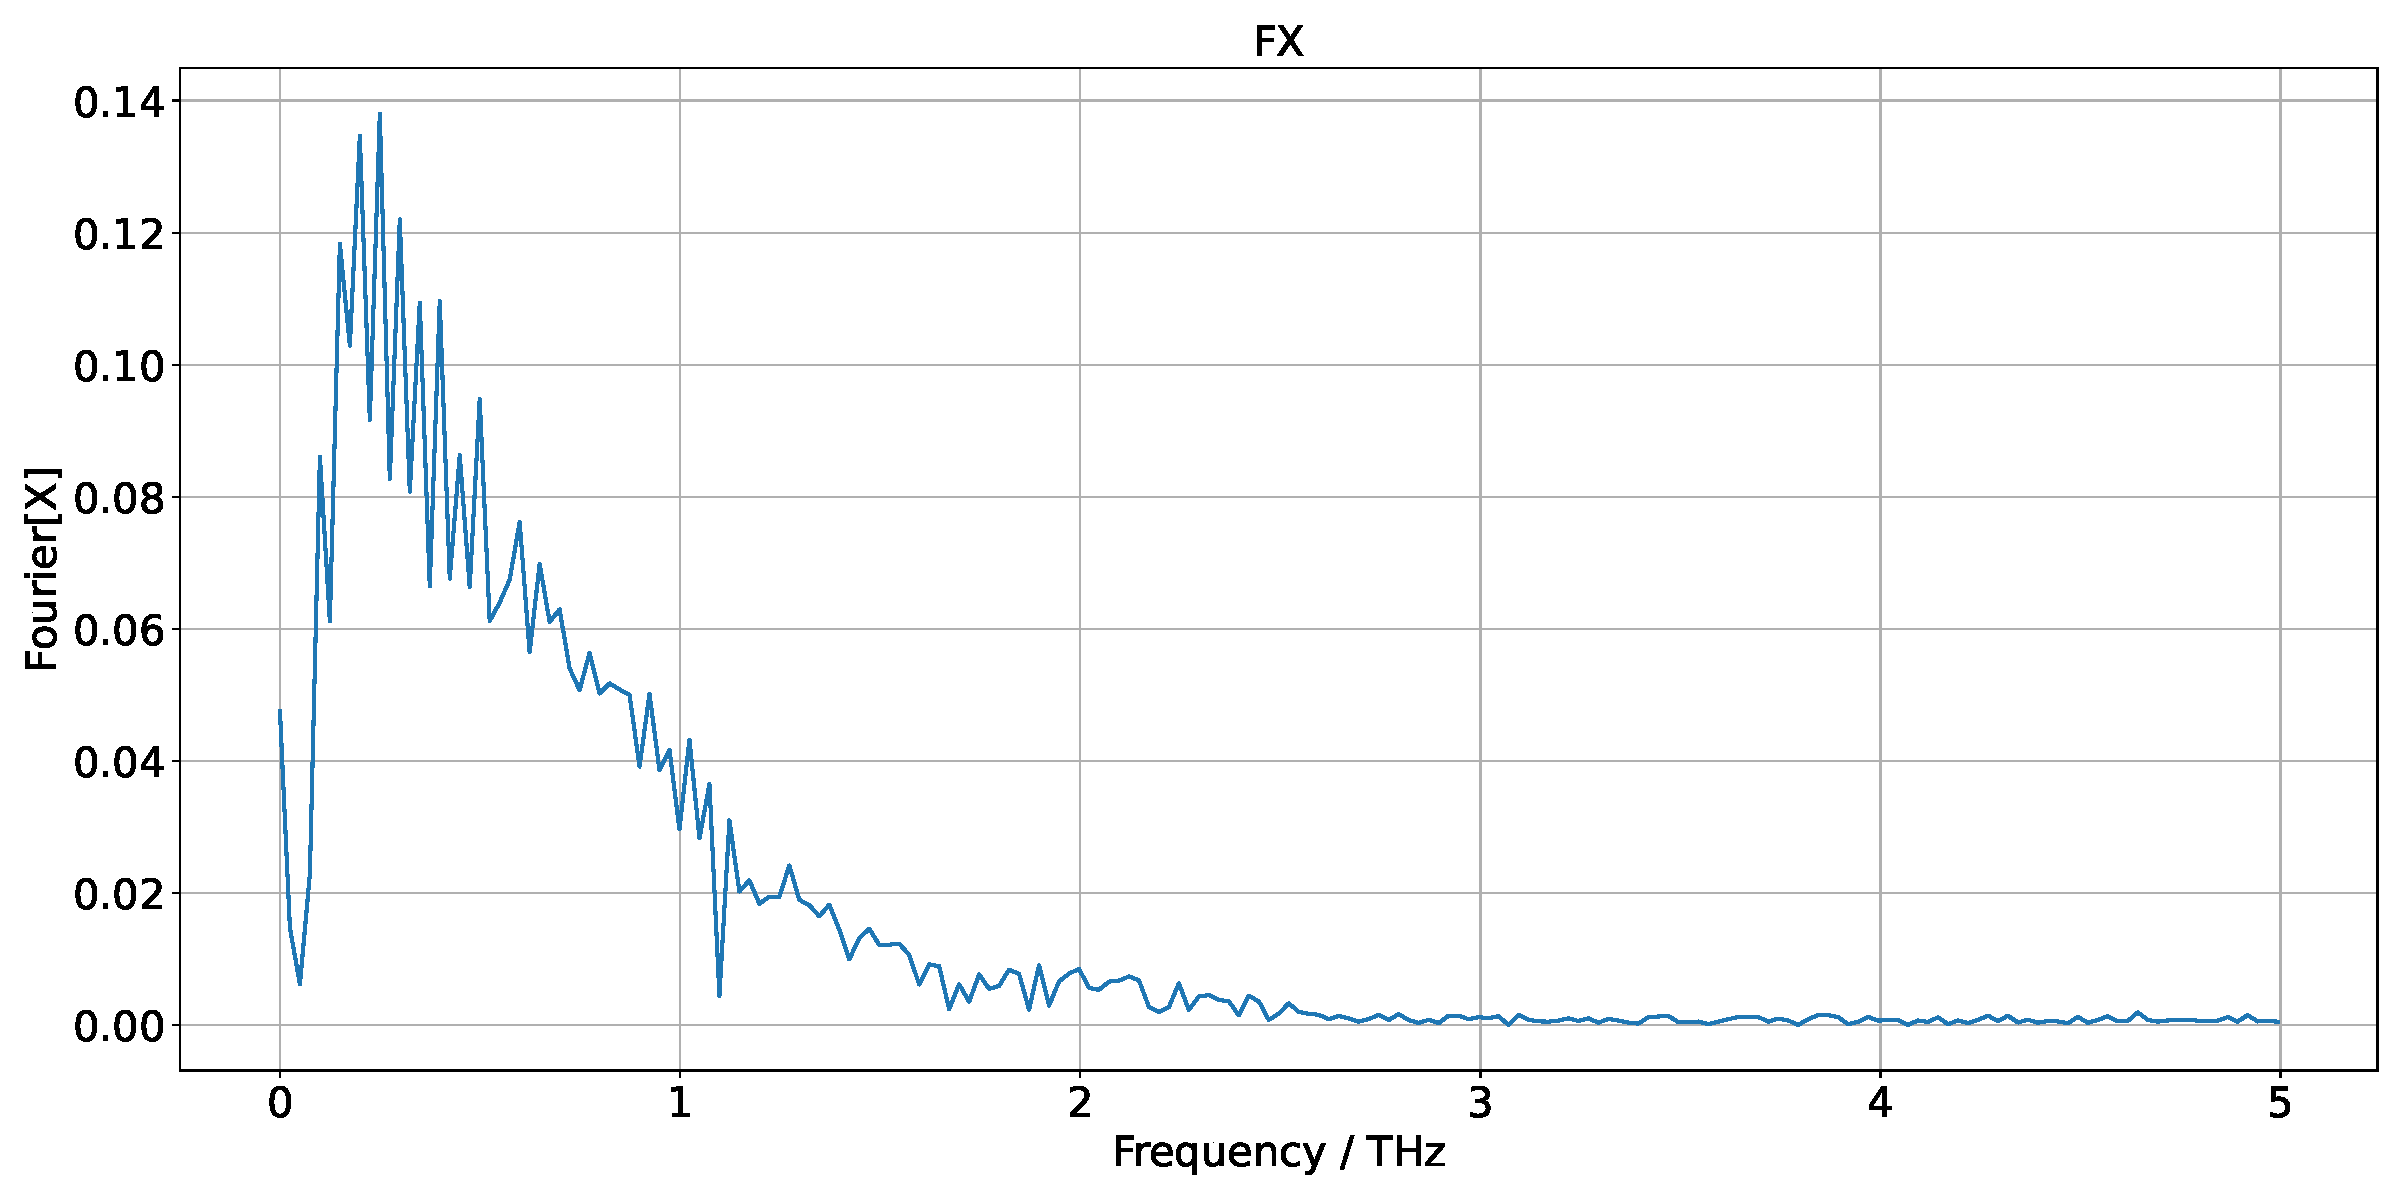
\includegraphics[width=\textwidth]{Plots/2_11_30_20normalFX.pdf}%
        \phantomsubcaption
    %    \caption{The Fourier-Transformation of the $\si{\tera\hertz}$ pulse that is shown in figure \ref{ZnTe:2_11_30_20_signal}.
    %    It can be seen that the frequency of the radiation lies in the lower $\si{\tera\hertz}$ regime.}%
        \label{fig:2_11_30_20_fft}%
    \end{subfigure}%
    \hfill% Fills available space in the center -> space between figures
    \begin{subfigure}{.55\textwidth}%
        \centering
        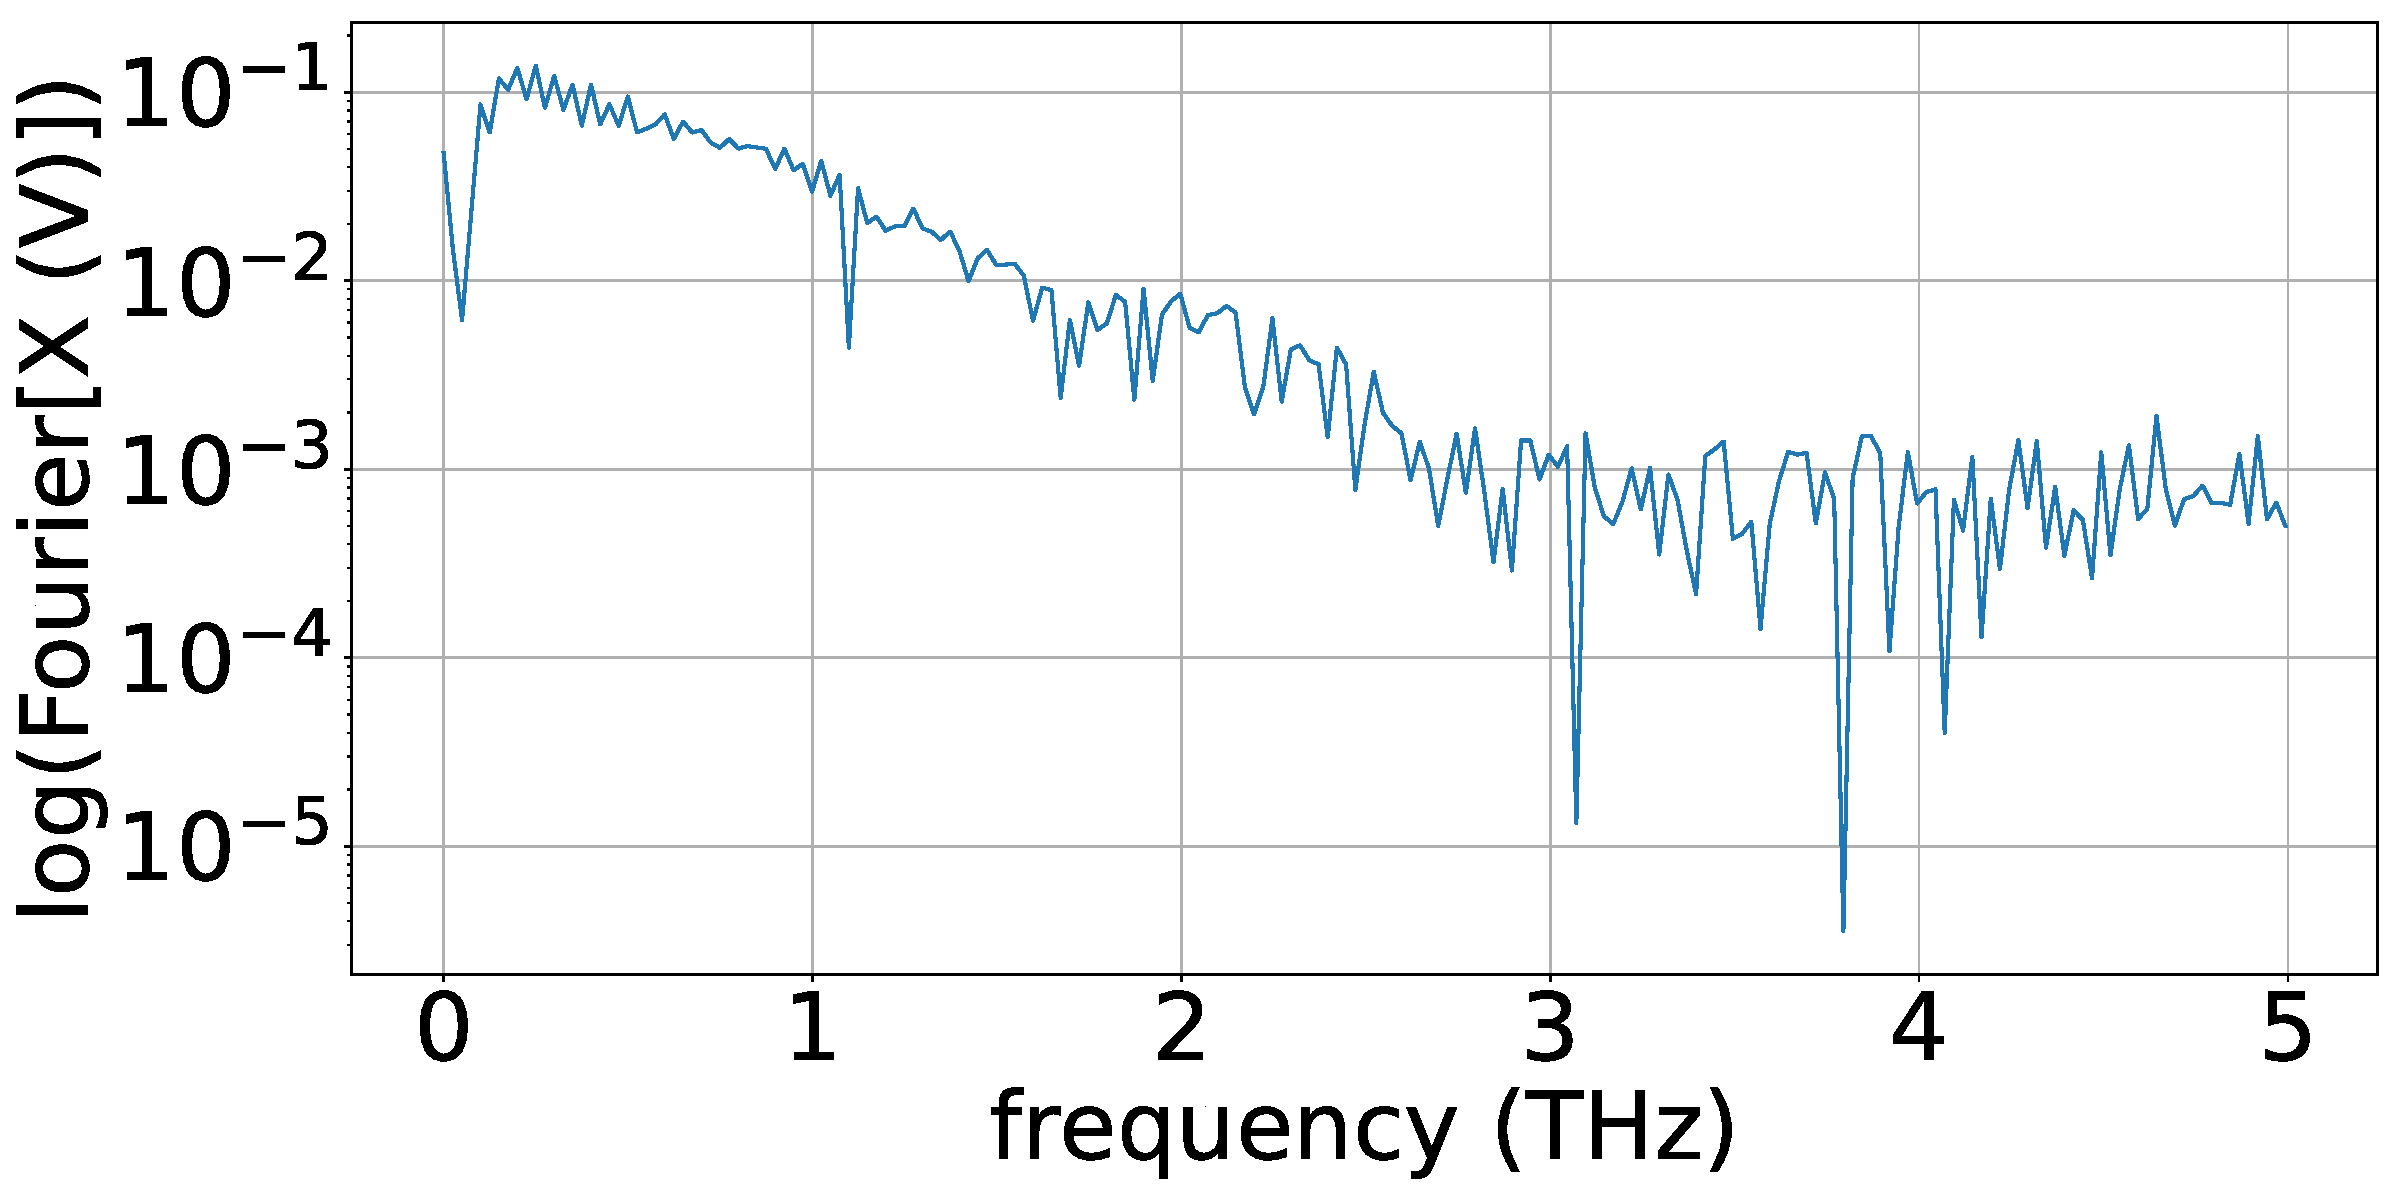
\includegraphics[width=\textwidth]{Plots/2_11_30_20normallog(FX).pdf}%
        \phantomsubcaption
 %       \caption{The Fourier spectrum of the data that is shown in figure \ref{ZnTe:2_11_30_20_signal} is plotted against a logarithmic y-axis.
  %      This shows that higher $\si{\tera\hertz}$ frequencies are generated as well. Some absorption lines can also be seen.}%
        \label{fig:2_11_30_20_fft_log}%
    \end{subfigure}%
    \caption{The Fourier spectrum of the data from ZnTe, which is collected with the highest pump power of $\SI{135.0}{\milli\W}$.
    The upper figure \ref{fig:2_11_30_20_fft} shows the Fourier spectrum of the $\si{\tera\hertz}$ radiation that is emitted by ZnTe, plotted against two linear axes.
    The lower Figure \ref{fig:2_11_30_20_fft_log} shows the spectrum plotted against a logarithmic y-axis to see the higher frequencies as well.}%
    \label{fig:fourier_znte}%
\end{figure}\FloatBarrier
\subsection{Electric field measurements}
\label{sec:znte_electricfield}
To determine the peak electric field of the $\si{\tera\hertz}$ pulse, several measurements of $A$, $B$ and $A-B$ are taken as described in section \ref{sec:field}.
To get the best results and minimize the error through noise for $A$ and $B$, their value is measured $500$ times.
This is done for the high initial laser power and the lower initial laser power.
After the data is taken, the mean values of $A$ and $B$ are calculated.
The uncertainty of $A$ and $B$ is the standard deviation.
\\
All further errors are calculated with the python package uncertainties \cite{uncertainties}, which uses standard error propagation theory.
With those, the electric field for every $A-B$ value is calculated by equation \eqref{eq:electricfield_A_B}.
All the peak electric field values are then collected and plotted against their corresponding pump power.
The resulting plot can be seen in figure \ref{fig:znte_electricfield}.\FloatBarrier
\begin{figure}
    \centering
    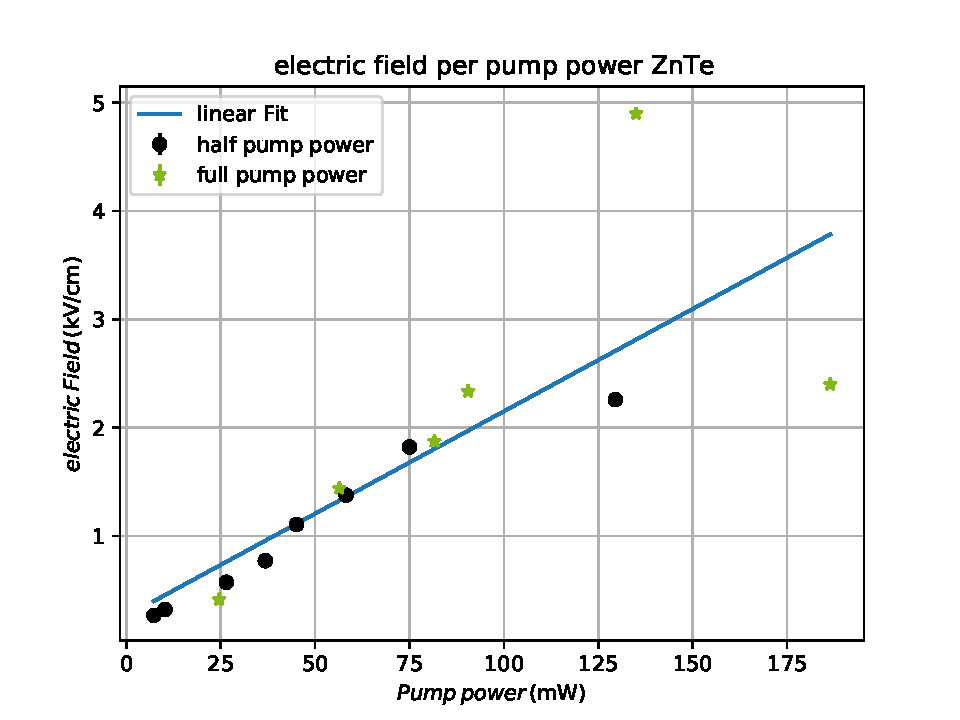
\includegraphics[width=0.65\textwidth]{Plots/eltric_field_ZnTe.pdf}
    \caption{The calculated peak electric fields of the $\si{\tera\hertz}$ pulse from ZnTe are plotted against their corresponding pump laser powers.
    Different initial laser powers are shown through different colors. The high power is $\SI{579}{\milli\W}$ the lower is $\SI{291}{\milli\W}$.}
    \label{fig:znte_electricfield}
\end{figure}\FloatBarrier
The laser changes its power from $\SI{291}{\milli\W}$ to $\SI{579}{\milli\W}$, over the course of the measurement. 
For this, the values measured with the higher initial laser power are marked with green stars.
The lower initial laser power of $\SI{291}{\milli\W}$ is marked with black dots.
%A linear regression is done with the formula
%\begin{equation}
%    f(x) = mx + b,
%    \laeqbel{eq:linear}
%\end{equation}
%where $x$ are the pump power values and $f(x)$ are all the peak electric field values.
%The calculation are done with the function \textbf{curve\_fit} from the python package scipy \cite{scipy}.
%It returns the fit parameters 
%\begin{align*}
%    m =& 0.0189\\
%    b =& 0.2615
%    vielleicht sollte ich kein align nutzen auch wenn es am besten aussieht. das nimmt einfach zu viel platz weg
%\end{align*}
%with which the linear fit is plotted.
The lower initial laser power electric fields show a linear trend, the same can be said for the higher initial laser power if looked at isolated.
However, the gradient of the higher initial laser power is less than that of the lower initial laser power.
\\\\
%The linear trend is in good comparison with the literature \cite{electric_field_compare} if just the lower initial pump power is looked at.
The maximum electric field strength that is calculated is $\SI{9.59(15)}{\kilo\V\per\centi\meter}$, which corresponds to a pump power of $\SI{129.5}{\milli\W}$.
This is not the highest pump power that is used.
The expectation would be that the highest pump power corresponds to the highest peak electric field.
The reason for this anomaly, as well as the lower field strengths at the higher initial laser power, might be that the beam path from the low and high power measurements diverge from one another.
This leads to a mismatch of the $\si{\tera\hertz}$ pump beam and the probe beam at the higher initial laser power.
Because the pump and probe beam are then not aligned properly, the probe beam polarization changes less in comparison to the lower initial pump power.

\FloatBarrier
\subsection{Power measurements}
\FloatBarrier
To calculate the peak electric field power of the $\si{\tera\hertz}$ pulse the spot size of the pulse on the detector is measured as described in section \ref{sec:power}.
The spot has a radius of $\SI{2.5}{\milli\meter}$ according to the aperture opening.
If a circular spot is assumed the spot area is $\SI{19.62}{\milli\meter\squared}$.
With the electric field values that are calculated in section \ref{sec:znte_electricfield}, the intensity can then be calculated according to equation \eqref{eq:intensity}.
Now all variables to calculate the $\si{\tera\hertz}$ electric field power are known and just need to be plugged into equation \eqref{eq:power}.
\\
The resulting power values are then plotted against their corresponding pump powers and shown in figure \ref{fig:znte_power}.\FloatBarrier
\begin{figure}
    \centering
    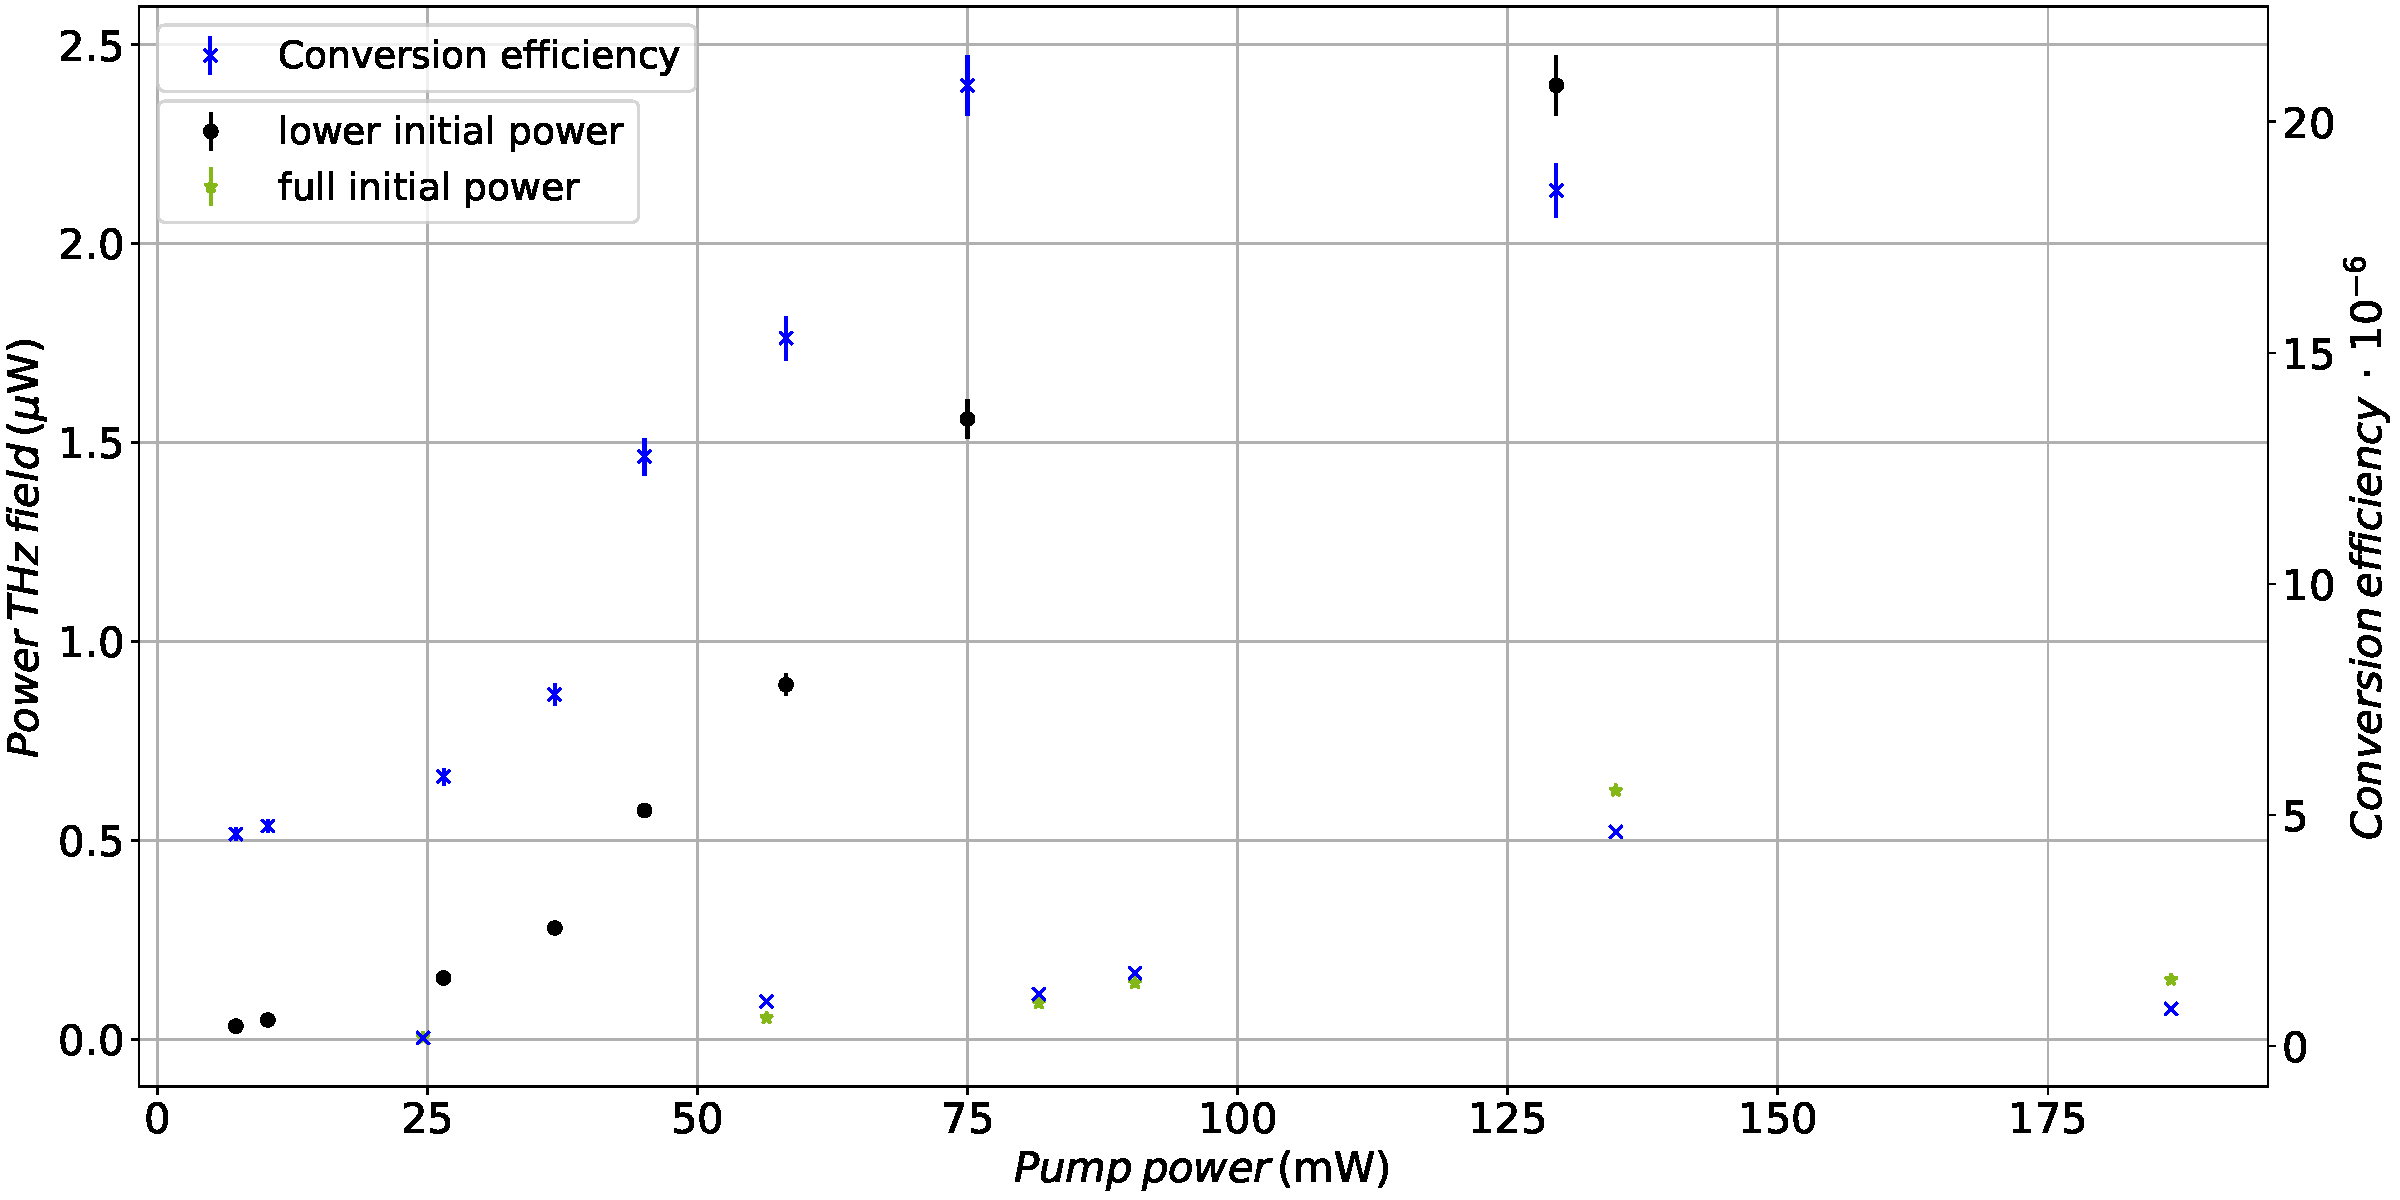
\includegraphics[width=0.8\textwidth]{Plots/Powerznte.pdf}
    \caption{The calculated peak electric field powers of the $\si{\tera\hertz}$ pulses from ZnTe are plotted against their corresponding pump powers.
    Because the initial laser powers that are fed into the setup change over the course of the measurement, the different laser powers are marked with green stars, for the higher power, or black dots, for the lower power.
    The high initial laser power has a value of $\SI{579}{\milli\W}$ and the lower a value of $\SI{291}{\milli\W}$.
    A conversion efficiency from pump power to $\si{\tera\hertz}$ power is calculated and shown as blue crosses. 
    The conversion efficiency is plotted against an additional y-axis, which is visible on the right side.}
    \label{fig:znte_power}
\end{figure}\FloatBarrier
Because the initial laser power that comes into the setup changes, the different laser powers are marked with green stars, for high power, and black dots, for lower power.
The high initial laser power has a value of $\SI{579}{\milli\W}$ and the lower a value of $\SI{291}{\milli\W}$.
\\
The conversion efficiency from laser pump power to $\si{\tera\hertz}$ peak electric field power is calculated and plotted as blue crosses in figure \ref{fig:znte_power}.
It is calculated via equation \eqref{eq:conversion}.
\\\\
Because the measurements of the low initial power and the high initial laser power diverge from one another, just the higher initial laser power is looked at first.
The calculated peak electric field powers of the $\si{\tera\hertz}$ pulse, show a low exponential growth which switches to a linear trend after about $\SI{50}{\milli\W}$.
The highest peak electric field power has a value of $\SI{2.389(75)}{\micro\W}$ at a pump power of $\SI{129.5}{\milli\W}$.
\\
The peak electric field powers for the high initial laser power also show a low exponential trend but reach a maximum at $\SI{135.0}{\milli\W}$, after which the power of the $\si{\tera\hertz}$ electric field drops again.
Their gradient is smaller than the gradient of the other dataset, with its highest peak electric field power being $\SI{0.626(4)}{\micro\W}$.
The reason for this divergence is the same as the one that influences the electric field strengths, as the peak electric field powers are calculated out of the field strengths.
%or maybe this would be the real behavior if the crystal is not burned. so that the power would rise linearly for even longer.
\\
Now to the lower initial laser power.
The conversion efficiency of the lower initial laser power shows a linear increasing trend with rising pump power.
It reaches its maximum at $\SI{75.0}{\milli\W}$ with its conversion efficiency being $\SI{2.08(7)e-05}{}$.
After a pump power of $\SI{75.0}{\milli\W}$, the conversion efficiency drops down a bit but stays almost constant.
A similar trend is seen in \cite{THZ_eltric_field}, where the conversion efficiency stays constant for increasing pulse energies per area.
The visible divergence can be explained by the lower crystal quality, due to its burned spots.
The lower initial laser power shows just very low conversion efficiencies and they are way under those presented in \cite{THZ_eltric_field}.
\\\\
A comparison of the peak electric field powers with the literature is quite hard because most other setups use pump powers that are higher than the ones reached in this setup.
However, the measurements of the $\si{\tera\hertz}$ energy from \cite{THZ_eltric_field} show a similar trend at low pulse energies per area.
\\
%The most probable reason for that are the burned parts of the crystal, that lowers the efficiency of the crystal.
%The conversion from pump power to pulse energy per unit area is also just a rough estimation because the laser power is not equally distrubuted over the laser spot, but rather follows a gaussian distrubution.
%It is to be expected that a lot of the laser power also does not even hit the crystal because the lens, that is positioned infront of the crystal, focuses the beam not enough for all the beam power to hit the crystal.
%This results in some laser power hitting the holder of the ZnTe crystal.
%The reason for not focusing down enough is to avoid reaching the damage threshold of the crystal as it is already damaged.
\FloatBarrier
\section{Gallium phosphide}
As the emitter crystal, a $\SI{0.3}{\milli\meter}$ GaP crystal is used.
A $\SI{1}{\milli\meter}$ ZnTe crystal is in use as the detector crystal.
The measurements and preparations are the same as for ZnTe and a detailed description can be found in section \ref{sec:execution}.
A first look at the data that is collected can be taken in figure \ref{fig:GaP14_55_42normalX}.\FloatBarrier
\begin{figure}
    \centering
    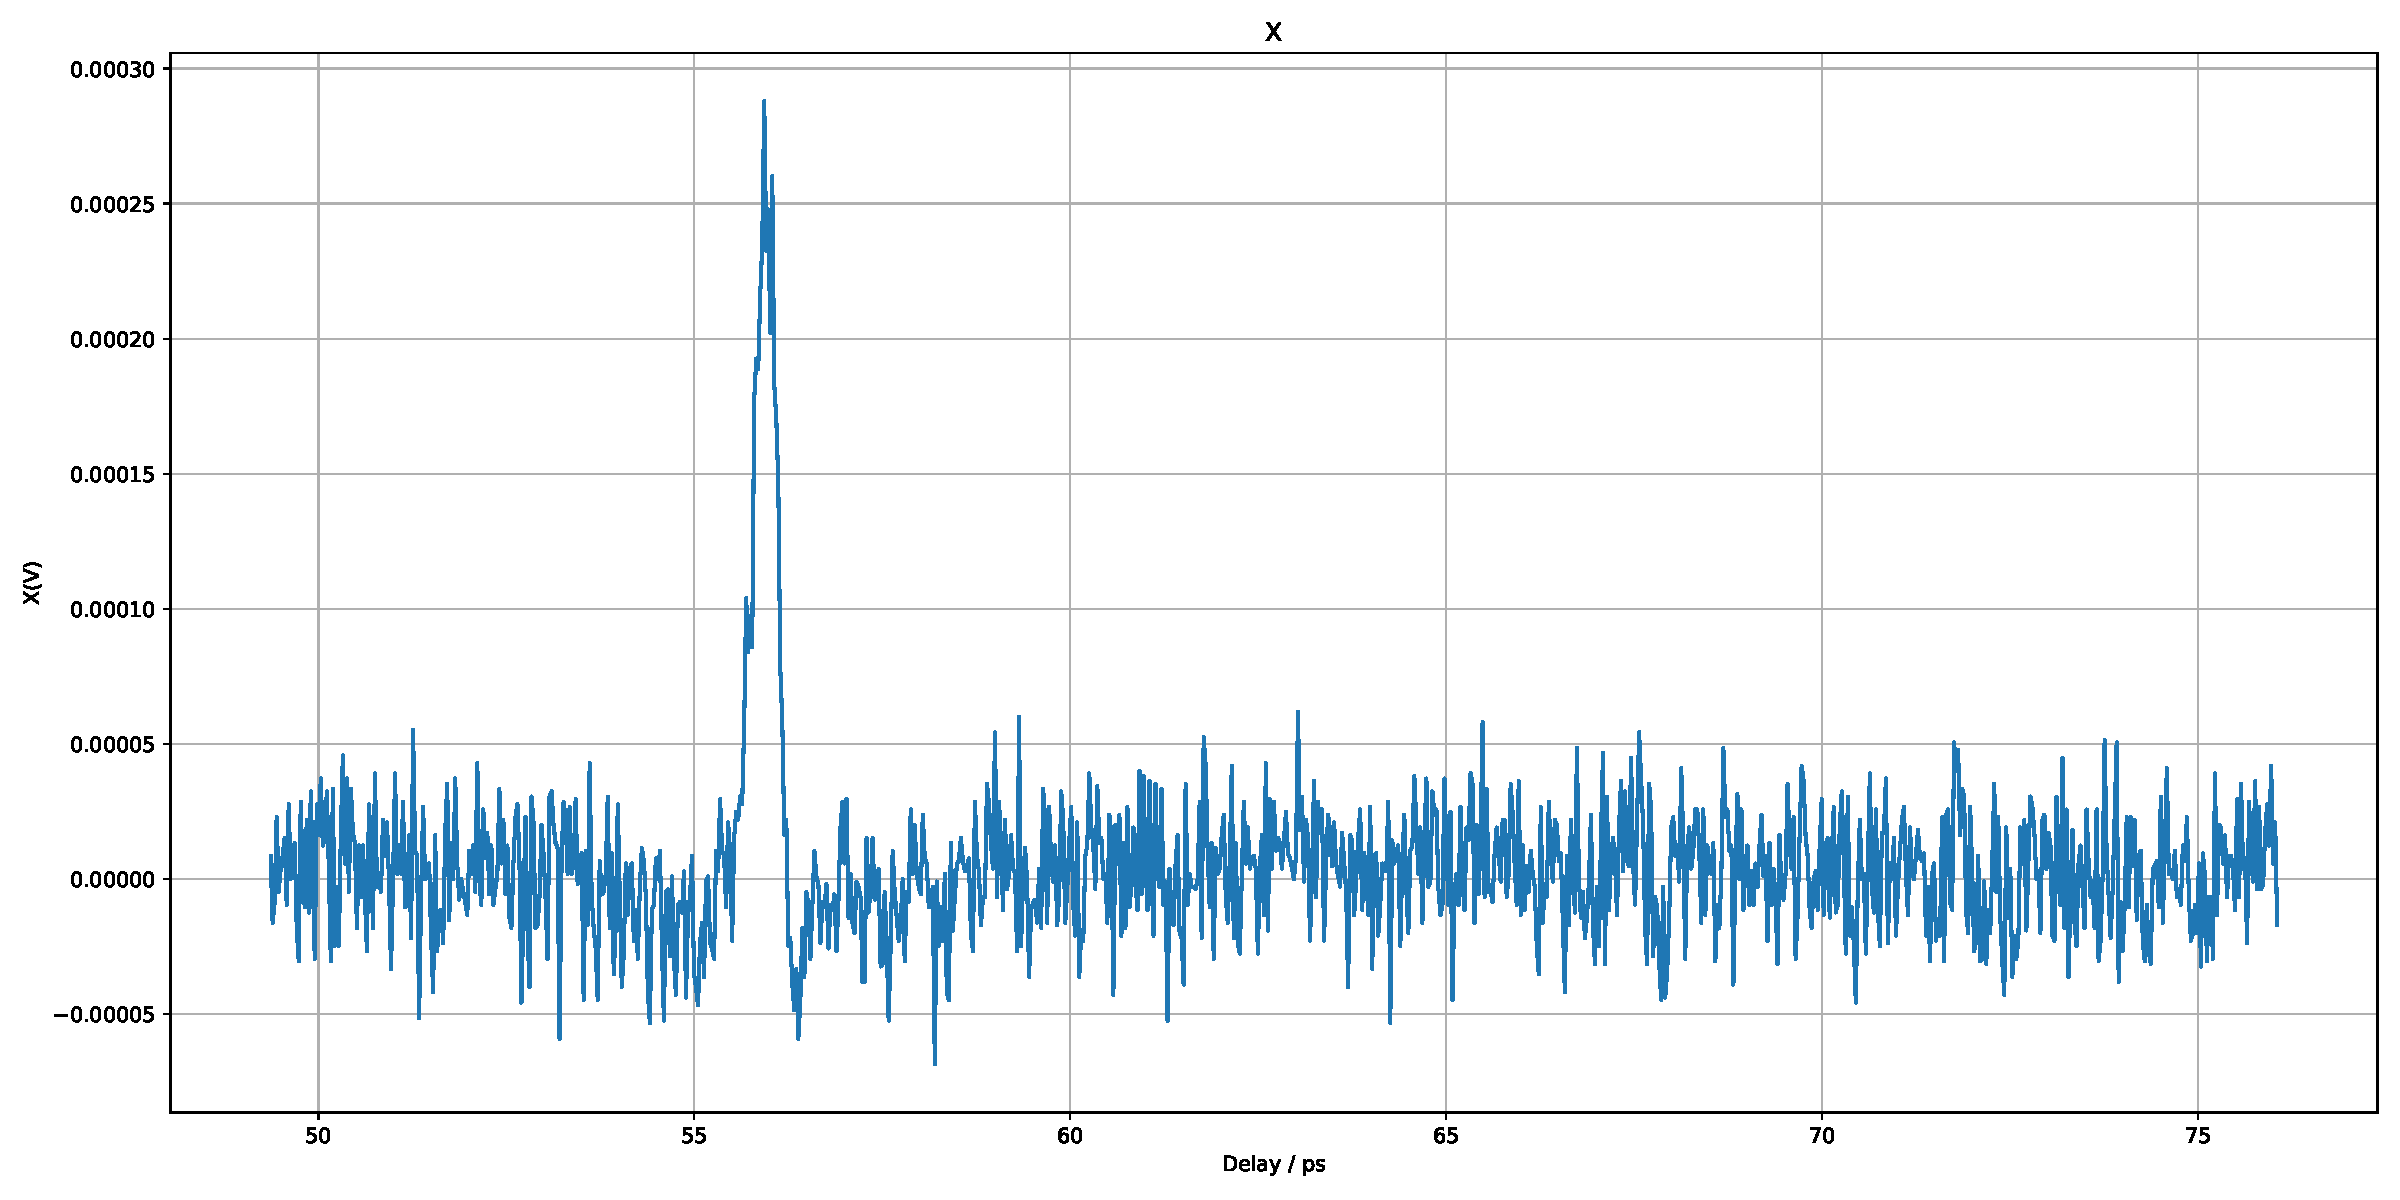
\includegraphics[width=0.8\textwidth]{Plots/GaP14_55_42normalX.pdf}
    \caption{The EOS data that is collected with GaP as emitter crystal with an applied laser pump power of $\SI{124.2}{\milli\W}$, which is the highest laser pump power that is used for GaP.}
    \label{fig:GaP14_55_42normalX}
\end{figure}\FloatBarrier
At the start of the measurement, the signal is distributed around zero, but not totally zero because of the noise.
Around $\SI{54}{\pico\second}$ a downward trend can be seen, which reaches its minimum at $\SI{55}{\pico\second}$.
Then the signal gradient becomes positive and increases in a very short interval up to a peak value of $\SI{0.287}{\milli\V}$ at a delay of $\SI{55.9}{\pico\second}$.
\\
After the peak, the signal drops down again to another minimum with a value of $\SI{-59.128}{\micro\V}$ at a delay of $\SI{56.3}{\pico\second}$.
Now the signal raises back to zero and shows no further significant features until the end of the measurement.
This measurement does not show any post pulse feature, probably because the noise is too high to see the post pulse.
\\\\
A Fourier-Transformation is calculated, which is shown in figure \ref{fig:GaP14_55_42_fft}.
The Fourier spectrum is also plotted against a logarithmic y-axis to make absorption lines more visible and acquire more information about the higher frequencies, that do not appear in the normal Fourier spectrum.
\\
The Fourier spectrum that is plotted against the logarithmic y-axis is shown in figure \ref{fig:GaP14_55_42_fft_log}.
There are no features in the Fourier spectrum that can be recognized as absorption lines.
The Fourier spectrum drops down from its highest amplitude at a frequency of $\SI{0.3}{\tera\hertz}$ to a frequency of $\SI{2.5}{\tera\hertz}$.
After $\SI{2.5}{\tera\hertz}$ the spectrum stays almost constant in amplitude, which shows that the majority of the generated radiation lies between $0.3$ and $\SI{2.5}{\tera\hertz}$.
\\
However, the low amplitude at higher frequencies could also be caused by the detection crystal.
As ZnTe has a phonon mode at $\SI{5.3}{\tera\hertz}$, which limits its ability to detect higher frequencies.
But because the amplitude of frequencies that are below the phonon mode is already low, it is more probable that the limitation lies at the emitter.
\begin{figure}%
    \centering
    \begin{subfigure}{.6\textwidth}%
        \centering
        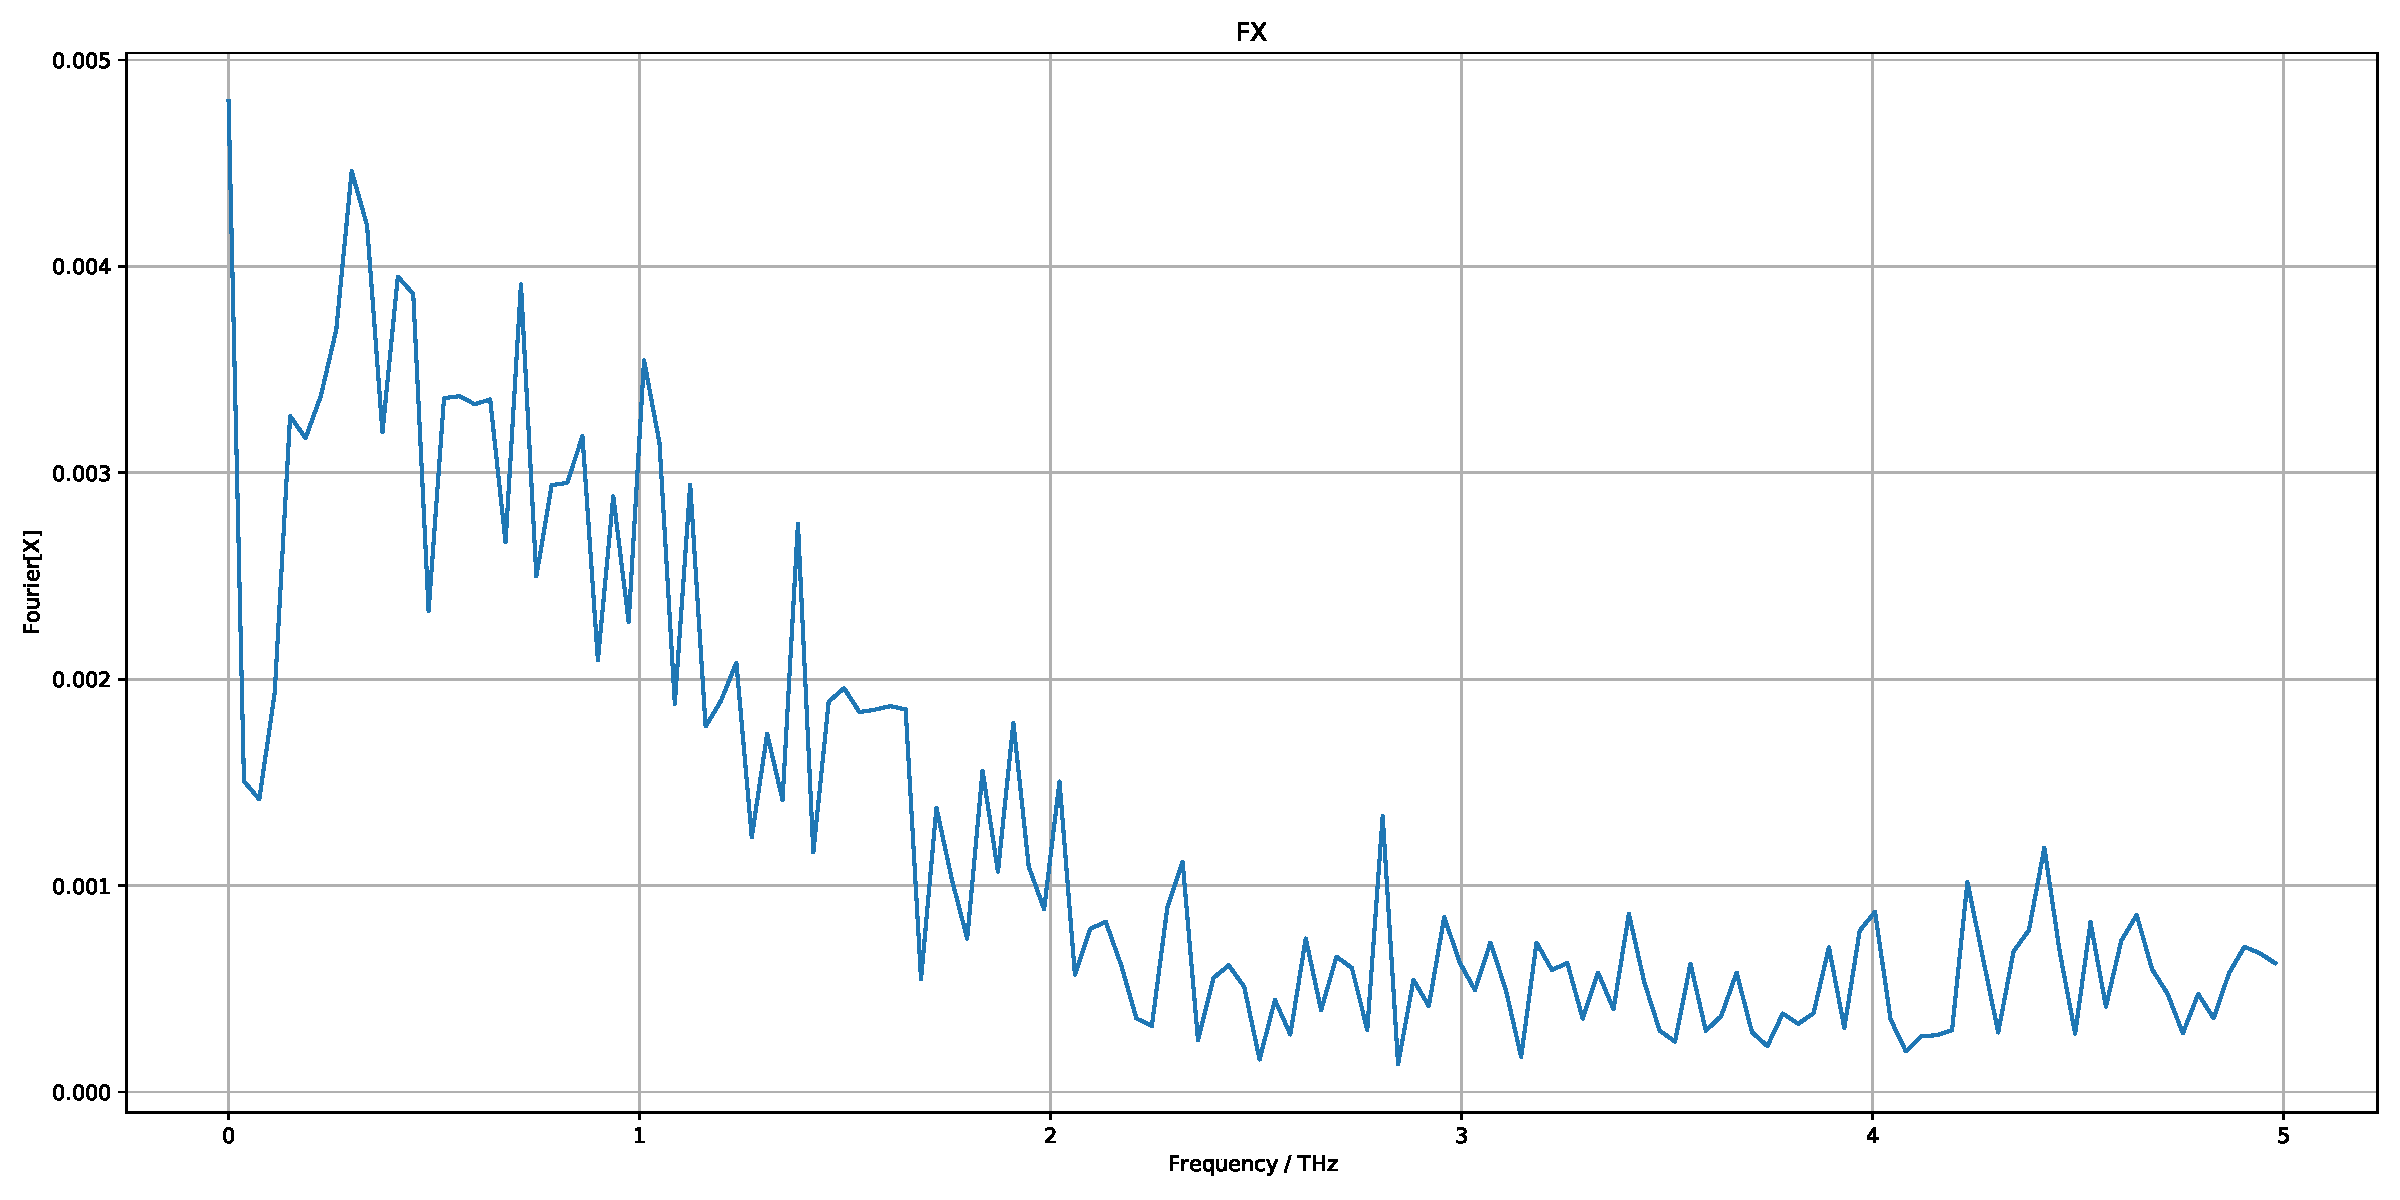
\includegraphics[width=\textwidth]{Plots/GaP14_55_42normalFX.pdf}%
        \phantomsubcaption
%        \caption{The Fourier-Transformation of the $\si{\tera\hertz}$ pulse from GaP shown in figure \ref{fig:GaP14_55_42normalX}.
%        The Fourier spectrum shows a linear downward trend from $\SI{0.3}{\tera\hertz}$ to $\SI{2.5}{\tera\hertz}$.
%        After which the spectrum stays almost constant.}%
        \label{fig:GaP14_55_42_fft}%
        \end{subfigure}%
    \hfill% Fills available space in the center -> space between figures
        \begin{subfigure}{.6\textwidth}%
        \centering
        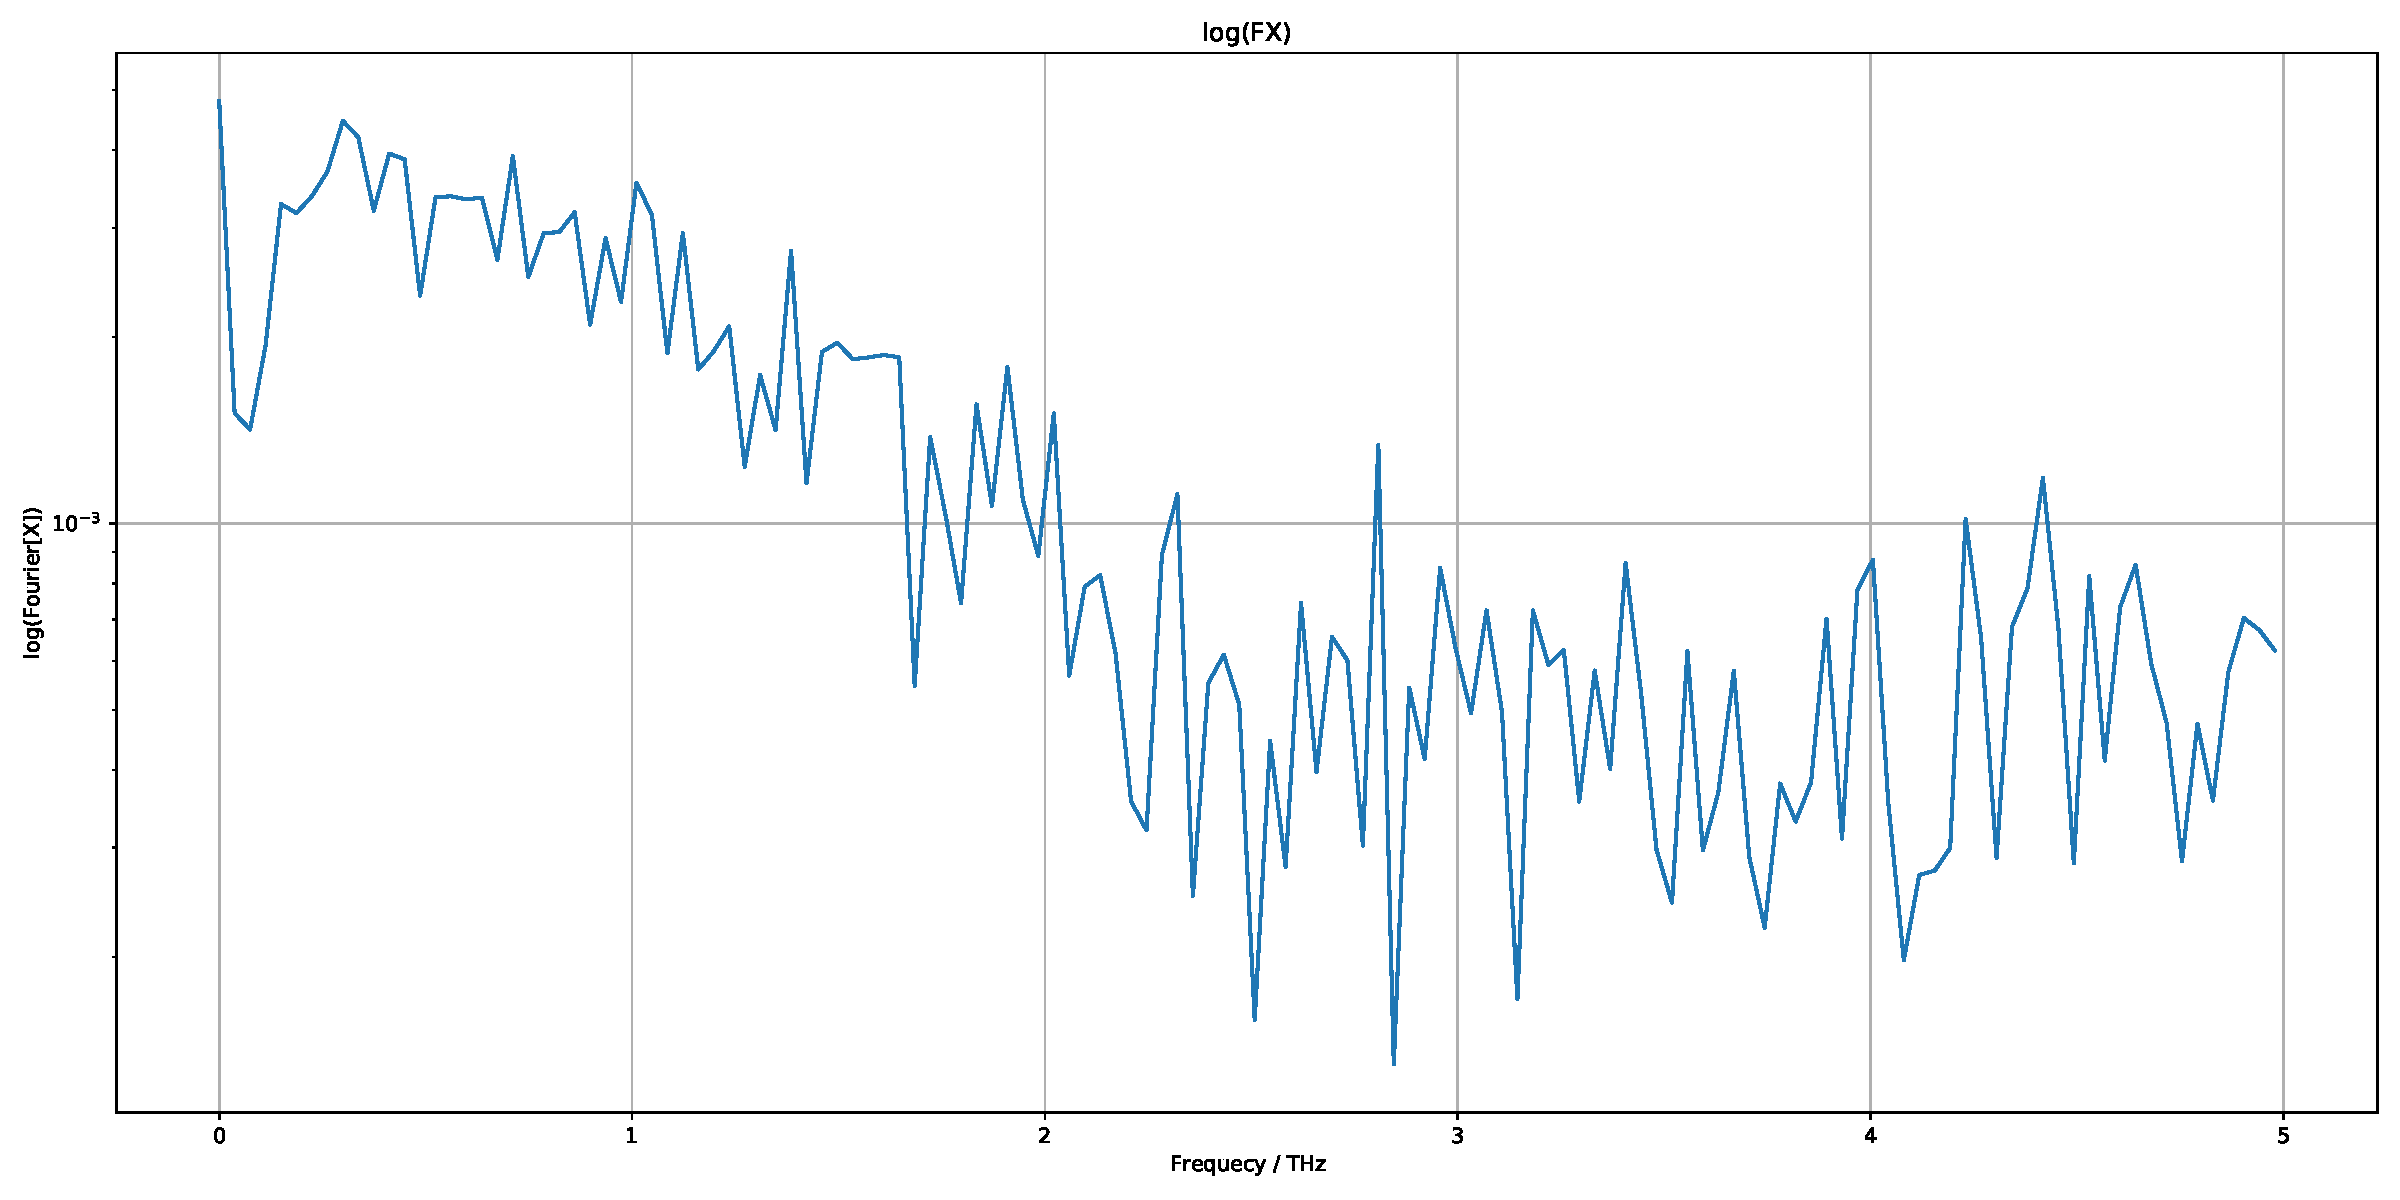
\includegraphics[width=\textwidth]{Plots/GaP14_55_42normallog(FX).pdf}%
        \phantomsubcaption
%        \caption{The Fourier spectrum of the GaP data is shown in figure \ref{fig:GaP14_55_42normalX}, plotted against a logarithmic y-axis.
%        There are no absorption lines recognizable in the plot.}%
        \label{fig:GaP14_55_42_fft_log}%
    \end{subfigure}%
    \caption{The Fourier spectrum of the data for GaP, shown in figure \ref{fig:GaP14_55_42normalX}, which is collected with the highest pump power of $\SI{124.2}{\milli\W}$.
    The upper figure \ref{fig:GaP14_55_42_fft} shows the $\si{\tera\hertz}$ Fourier spectrum emitted by GaP which is plotted against two linear axes.
    The lower figure \ref{fig:GaP14_55_42_fft_log} shows the Fourier spectrum plotted against a logarithmic y-axis.}%
    \label{fig:fourier_gap}%
\end{figure}%
\FloatBarrier
\subsection{Electric field measurements}
\FloatBarrier
The electric field is measured as described in section \ref{sec:field}.
To calculate the peak electric field, the positive peak $A-B$ values, which are taken by each measurement are plugged into equation \eqref{eq:electricfield_A_B}.
The peak electric fields for every pump power are then plotted against their corresponding pump powers.
The resulting plot is shown in figure \ref{fig:gap_electricfield}.\FloatBarrier
\begin{figure}
    \centering
    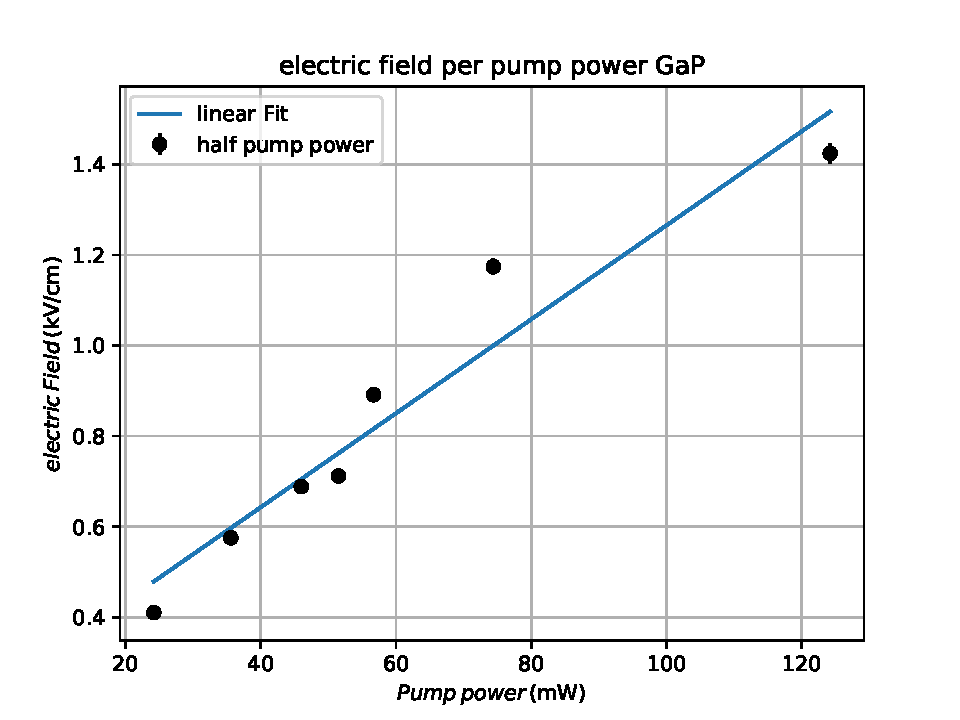
\includegraphics[width=0.65\textwidth]{Plots/eltric_field_GaP.pdf}
    \caption{The peak electric fields of GaP, marked as black dots, are plotted against their corresponding pump powers.
    A linear fit, as filled blue line, for the plotted data points are also shown in the figure.
    The fit parameter is its gradient with $m=\SI{0.0245(30)}{\kilo\V\per\milli\W\centi\meter}$ and the y-axis crossing at $b=\SI{0.5403(2002)}{\kilo\V\per\centi\meter}$.}
    \label{fig:gap_electricfield}
\end{figure}\FloatBarrier
The calculated peak electric fields show a linear trend.
For this reason a linear regression is calculated for equation  
\begin{equation}
    f(x) = mx+b \,.
\end{equation}
The regression is done with the function \textbf{curve\_fit} from the python package scipy.
Said function returns the parameters
\begin{align*} 
    m &= \SI{0.0245(30)}{\kilo\V\per\milli\W\centi\meter}\\
    b &= \SI{0.5403(2002)}{\kilo\V\per\centi\meter}
\end{align*}
which are used to make the linear fit shown in figure \ref{fig:gap_electricfield}.
\\
The linear regression confirms that the data points follow a linear trend.
At higher pump powers the data points are more distant from the linear fit.
The highest electric field of $\SI{3.38(5)}{\kilo\V\per\centi\meter}$ that is calculated, corresponds to a pump power of $\SI{124.2}{\milli\W}$, which is the highest laser pump power that is used.
\FloatBarrier
\subsection{Power measurements}
Out of the peak electric fields of the $\si{\tera\hertz}$ radiation, the peak power can be estimated.
For this, the intensity $I$, defined in equation \ref{eq:intensity}, needs to be determined first.
\\
Additionally to the intensity, the area of the $\si{\tera\hertz}$ spot on the detector crystal needs to be measured.
How the spot size is determined is explained in section \ref{sec:power}.
The spot size has an estimated area of $\SI{19.62}{\milli\meter\squared}$.
The power is then calculated with equation \eqref{eq:power}, and the resulting values for the peak electric field powers are shown in figure \ref{fig:gap_power}.\FloatBarrier
\begin{figure}
    \centering
    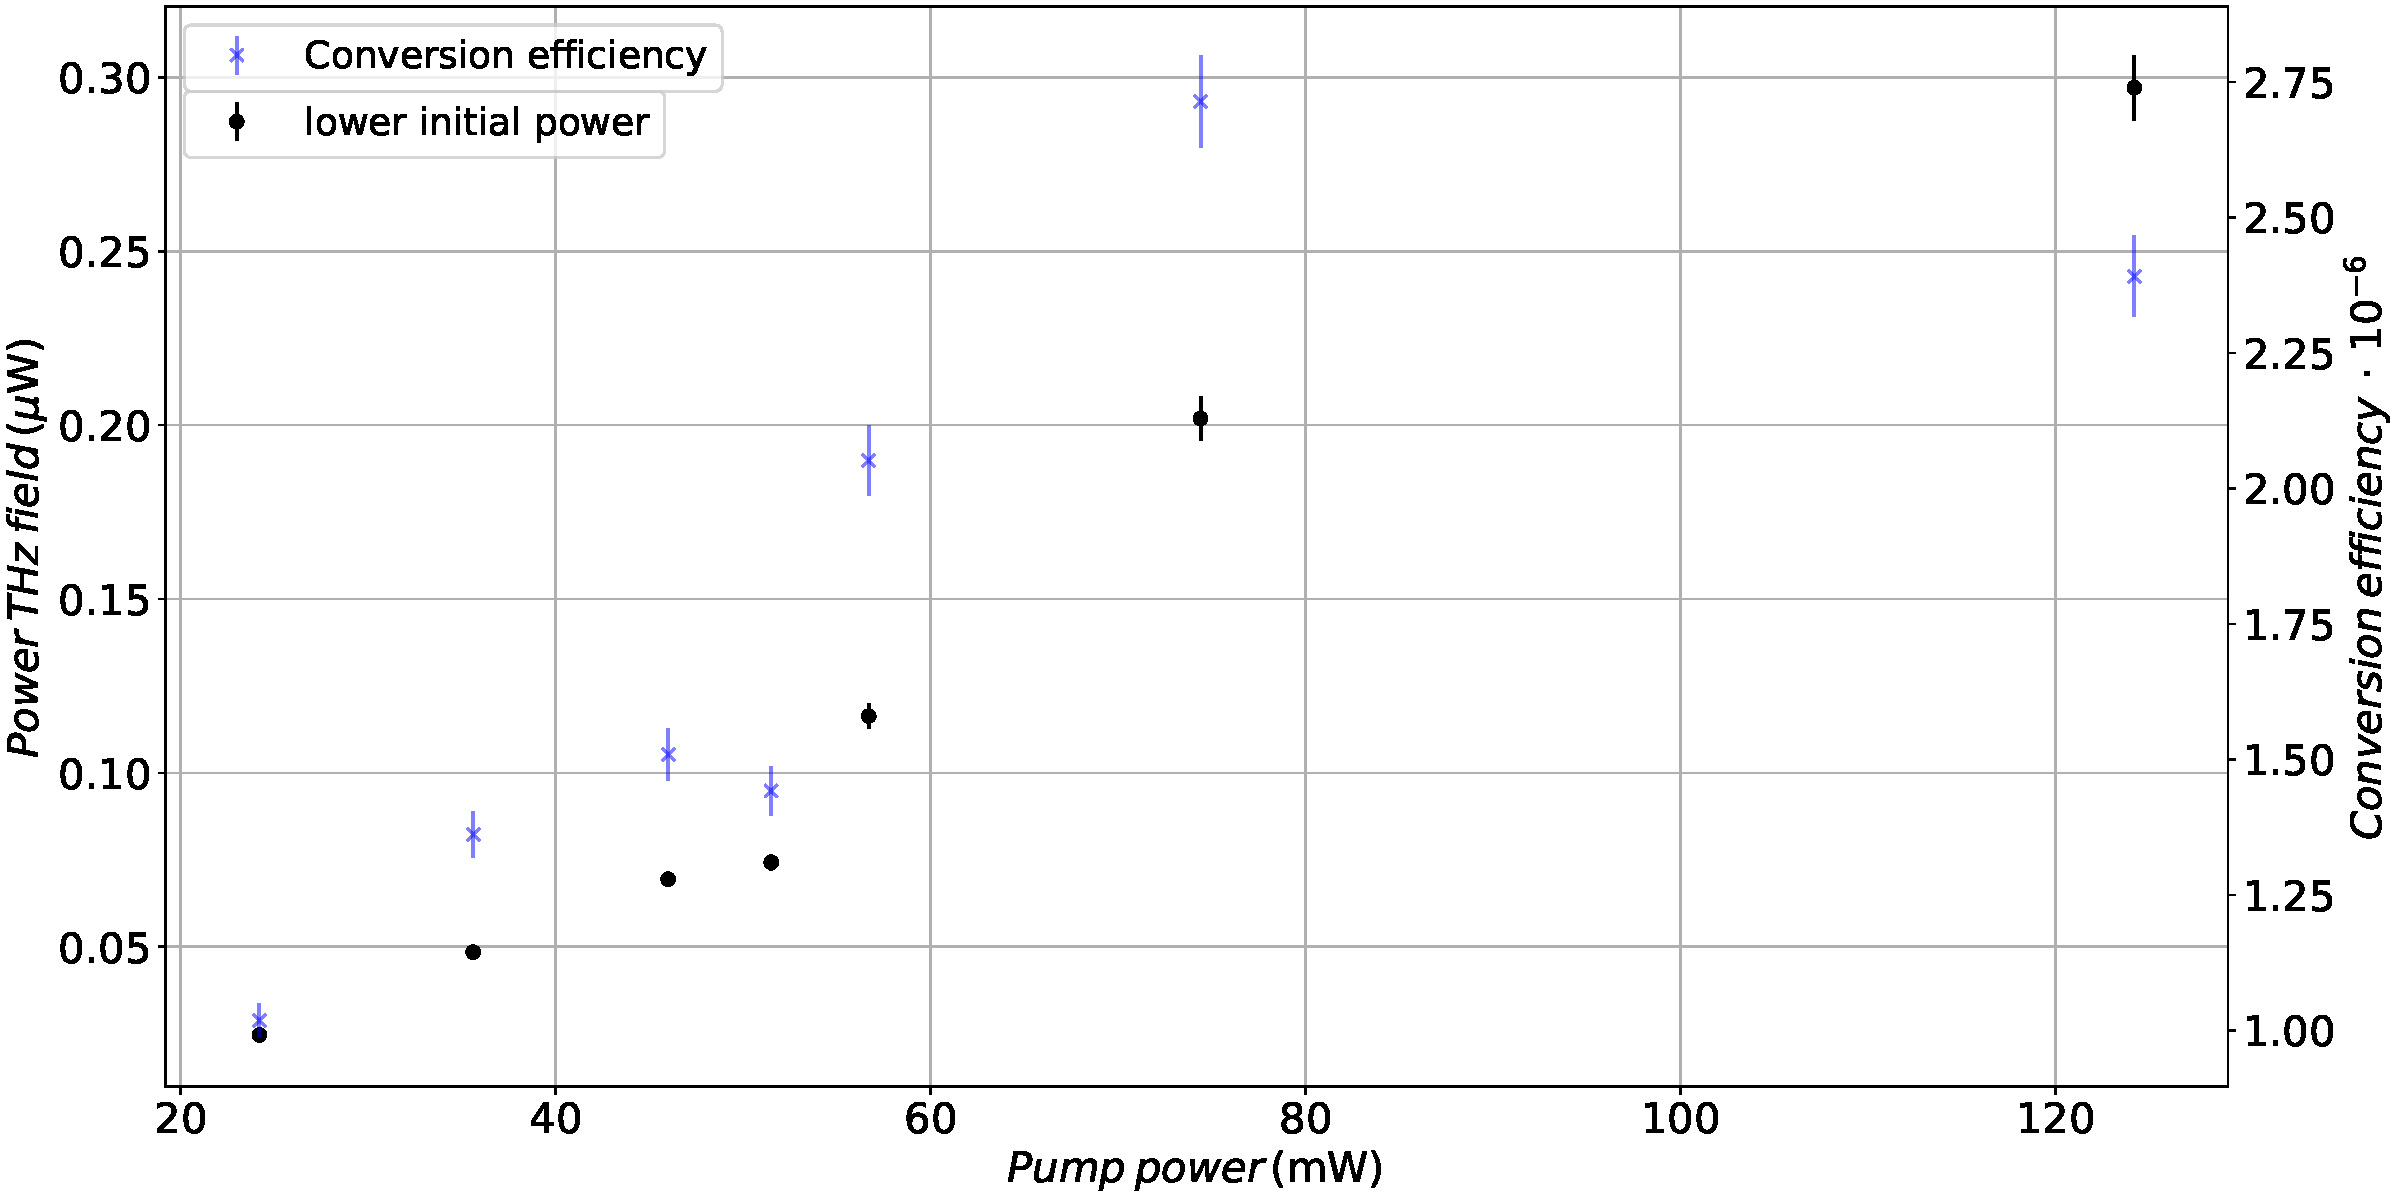
\includegraphics[width=0.8\textwidth]{Plots/Powergap.pdf}
    \caption{The calculated peak electric field powers for GaP are plotted against their corresponding pump powers, as black dots.
    The conversion efficiency, for each pump power, is calculated and also plotted against an additional y-axis on the right side.
    The conversion efficiency is shown as blue crosses.}
    \label{fig:gap_power}\FloatBarrier
\end{figure}
In this figure the peak electric field powers are plotted against their corresponding pump powers.
\\\\
The peak $\si{\tera\hertz}$ electric field powers of GaP show a low exponential growth which switches to a linear trend after about $\SI{50}{\milli\W}$, with its maximum being $\SI{0.297(9)}{\micro\W}$ at a pump power of $\SI{124.2}{\milli\W}$, which is the highest pump power that is used.
Between $40$ and $60 \, \si{\milli\W}$ pump power the linear trend seems to stagnate.
\\
The conversion efficiency seems to follow a similar linear trend, with there also being a negative gradient between  $40$ and $60 \, \si{\milli\W}$.
It already reaches its maximum at a pump power of $\SI{74.4}{\milli\W}$ with the conversion efficiency being $\SI{2.71(8)e-6}{}$.
At the higher pump power of $\SI{124.2}{\milli\W}$, the conversion efficiency drops down a bit to a value of $\SI{2.39(7)e-6}{}$.
It seems like there is a stagnation in the gradient of the conversion efficiencies at this pump power, but this can only be determined with more measurements.
\FloatBarrier
\section{Comparison}
Because the GaP crystal is $\SI{0.7}{\milli\meter}$ thinner than the ZnTe crystal all comparisons that are done in this chapter only apply to this specific setup and may not apply universally.
\\
The collected EOS signal from both ZnTe and GaP show a significant peak.
Before and after the peak, both signals show a small dip into the negative $A-B$ values.
The highest signal-to-noise ratio of ZnTe is higher than that of GaP, with it having a signal-to-noise ratio of $104/1$, while GaP has a signal-to-noise ratio of $14/1$, which is due to the smaller thickness of the GaP crystal that does not generate such high $\si{\tera\hertz}$ electric fields.
The signal to noise is calculated by 
\begin{equation}
    SNR = \frac{P_\text{signal}}{\sigma_\text{noise}}
\end{equation}
where $P_\text{signal}$ is the peak of the signal and $\sigma_\text{noise}$ is the standard deviation of the noise.
Furthermore, the signal-to-noise ratio of the lowest pump power with GaP goes down to $4.48/1$, which EOS signal can be seen in figure \ref{fig:GaP_noise}.
The oscillation after the pulse that is seen with the ZnTe crystal is strong and identifiable.
This is not the case for GaP, as the EOS signal is too noisy.
Furthermore, does the GaP EOS not show a post pulse, the most likely reason for this is that it is not distinguishable from the noise.
\\\\
The Fourier spectrum shows that ZnTe and the GaP crystal, generate $\si{\tera\hertz}$ radiation with most of it having frequencies between $0.3$ and $\SI{2}{\tera\hertz}$.
Moreover, in the ZnTe spectrum an absorption line can be seen, which is not the case with GaP, neither the logarithmic nor the normal Fourier spectrum show absorption lines.
Besides that, the GaP Spectrum seems to be more broadband than the ZnTe crystal, to confirm that more precise measurements with lower noise are necessary.
\\\\
The electric field strength of both crystals shows a linear dependency on the pump power, which shows no saturation at the power levels used.
However, the measured data from ZnTe shows some contradictory results, with its reason most likely being the switch to the higher initial pump power, which altered the pump beam path.
In further comparison, just the lower initial laser power will be examined.
The maximum generated electric field of ZnTe is about three times larger than that of GaP, even though the pump powers are almost the same with GaP at $\SI{124.2}{\milli\W}$ and ZnTe at $\SI{129.5}{\milli\W}$.
\\\\
At low pump powers, the power of the generated $\si{\tera\hertz}$ radiation of ZnTe shows an exponential trend, which GaP does not show.
Both follow a linear trend at pump powers between $50$ and $\SI{80}{\milli\W}$ after which both of their gradients lowers.
This behavior can also be seen in the conversion efficiency as it is the derivation of the peak $\si{\tera\hertz}$ power with respect to the pump power.
However, the peak conversion efficiency of ZnTe is about $7.5$ times higher than that of GaP. 

\end{document}
